\documentclass[11pt]{article}

% ---------- Portable preprint preamble (standard CTAN packages only) ----------
\usepackage[margin=1in]{geometry}
\usepackage[T1]{fontenc}
\usepackage{lmodern}
\usepackage{microtype}
\usepackage{amsmath,amssymb}
\usepackage{graphicx}
\usepackage{booktabs}
\usepackage{tabularx}
\usepackage{array}
\usepackage{caption}
\usepackage{xcolor}
\usepackage{enumitem}
\usepackage{authblk}
\usepackage{fancyhdr}
\usepackage[round]{natbib}
\usepackage[colorlinks=true,linkcolor=blue!55!black,citecolor=blue!45!black,urlcolor=blue!55!black]{hyperref}

\captionsetup{font=small,labelfont=bf}
\setlength{\parskip}{0.35em}
\renewcommand{\arraystretch}{1.15}
\newcolumntype{Y}{>{\raggedright\arraybackslash}X}

\pagestyle{fancy}
\fancyhf{}
\fancyhead[L]{\footnotesize Preprint --- M-PAPI companion to \emph{AI-Proliferation and Middle Powers}}
\fancyhead[R]{\footnotesize\thepage}
\renewcommand{\headrulewidth}{0.4pt}

\title{\textbf{Operationalising the Three-Axes Framework:\\ A Composite-Indicator Companion to\\ \emph{AI-Proliferation and Middle Powers}}}
\author[]{James Teague \and Alina Ali \and Sophie Sfeir \and Kristina Fort}
\affil[]{\small Companion to the working paper \emph{AI-Proliferation and Middle Powers: Preparation and Response Mechanisms} (2026)}
\date{\today}

\begin{document}
\maketitle
\thispagestyle{fancy}

\begin{abstract}
\noindent The working paper \emph{AI-Proliferation and Middle Powers} argues that fourteen named middle powers differ along three axes---\emph{capacity depth}, \emph{governance orientation}, and \emph{infrastructure posture}---and that the tractability of preparedness actions depends on a country's position along them, yet it never empirically positions any country. This companion study closes that gap with the Middle-Power AI-Proliferation Preparedness Index (M-PAPI): a reproducible composite indicator built from fourteen publicly sourced indicators following the OECD/JRC \emph{Handbook on Constructing Composite Indicators}. We report a literature-weighted ranking in which South Korea ($2.238$) and the United Kingdom ($2.178$) co-lead---Korea first under the equal and literature schemes, the UK first under PCA---and India ($0.103$) and Taiwan ($0.060$) trail; the top-five set $\{$UK, Korea, France, EU, Japan$\}$ is identical across equal-, PCA-, and literature-weighting schemes. Six hypotheses are pre-registered with numeric pass criteria and resolved mechanically: two are fully supported (cluster heterogeneity; insensitivity of the top tier to any single analyst-coded indicator) and four are partially supported with specific, named caveats (cross-axis separability, axis dimensionality, ranking robustness, and tier-membership stability). A vulnerability overlay maps axis scores onto the paper's three attack vectors, and counterfactual scenarios quantify per-country policy leverage. The ranking is strongly rank-concordant with the independent Oxford Insights Government AI Readiness Index 2024 (Spearman $\rho=0.863$ over the thirteen jurisdictions both cover), evidence of external concurrent validity. All outputs regenerate byte-for-byte under a pinned seed and an offline data snapshot. The index empirically grounds the paper's $\S$1--$\S$2 premise---the middle powers are differentiable, and the most-exposed tier is identifiable---while explicitly declining the $\S$3--$\S$4 claims it cannot yet test.
\end{abstract}

\noindent\textbf{Keywords:} composite indicators; AI governance; middle powers; AI proliferation; reproducible research; sensitivity analysis.

\tableofcontents

% ============================================================
\section{Introduction}
% ============================================================
The development of frontier artificial intelligence is concentrated in a small number of laboratories in the United States and China, leaving \emph{middle powers}---states with meaningful but non-dominant international influence---largely in the position of responding to, rather than shaping, the technology's trajectory. The working paper \emph{AI-Proliferation and Middle Powers: Preparation and Response Mechanisms} \citep{teague2026middlepowers} argues that, as access to highly capable model weights diffuses, middle powers face a structurally under-addressed vulnerability to three proliferation-enabled attack vectors---cyber-attacks, chemical/biological/radiological/nuclear (CBRN) threats, and influence operations---and that national-level preparedness is a more tractable priority than contesting the frontier. To organise that argument the paper distils two widely cited ``building blocks of AI power'' frameworks into three axes along which middle powers differ: \emph{capacity depth}, \emph{governance orientation}, and \emph{infrastructure posture}.

The paper names fourteen middle powers---the United Kingdom, Canada, France, Germany, Japan, India, Israel, Singapore, South Korea, Sweden, Saudi Arabia, the United Arab Emirates, the European Union, and Taiwan \citep{wang2024geopolitics}---and repeatedly invokes ``tractability depending on a country's position within the three axes,'' but it never \emph{positions} any country on those axes. This companion study supplies that missing empirical layer.

\paragraph{Contribution.} We construct the Middle-Power AI-Proliferation Preparedness Index (M-PAPI), a transparent composite indicator that places each of the fourteen middle powers on the three axes using fourteen publicly available indicators, and we report per-country rankings, a per-vector vulnerability overlay, and counterfactual policy scenarios. The study is deliberately \emph{not} new theory; it is empirical scaffolding that makes the working paper's per-country claims auditable, replicable, and updatable. We follow the OECD/JRC \emph{Handbook on Constructing Composite Indicators} \citep{oecd2008handbook} throughout and report three weighting schemes side by side with a full sensitivity battery.

\paragraph{Scope.} M-PAPI operationalises the paper's $\S$1 (axes and country set) and $\S$2 (attack vectors) only. The paper's $\S$3 (trigger-event ladder) and $\S$4 (detection/escalation/mitigation checklist) are \emph{not} operationalised: a country-year, AI-attributed incident dataset would be required for $\S$3, and the $\S$4 actions appear here only as the counterfactual policy scenarios of Section~\ref{sec:results}, not as country-year preparedness outcomes. The index measures \emph{relative} position within the fourteen-country reference frame; it does not claim that a high score means a country is ``safe.''

\paragraph{Pre-registration.} Six falsifiable hypotheses (H1--H6) are stated with numeric pass criteria before estimation (Table~\ref{tab:hyp}) and resolved mechanically against those criteria. Reporting the partial-support outcomes explicitly---rather than only the favourable ones---is a deliberate feature of the design.

% ============================================================
\section{Conceptual framework}\label{sec:framework}
% ============================================================
\subsection{The three axes}
Table~\ref{tab:axes} reproduces the paper's axis definitions and lists the indicators assigned to each. The fourteen indicators comprise five \emph{capacity-depth} measures, five \emph{governance-orientation} measures, and four \emph{infrastructure-posture} measures.

\begin{table}[t]
\centering
\caption{The three axes of the working paper's framework and the M-PAPI indicators assigned to each. Indicator construction and sources are detailed in Section~\ref{sec:data}.}
\label{tab:axes}
\footnotesize
\begin{tabularx}{\textwidth}{@{}l Y Y@{}}
\toprule
\textbf{Axis} & \textbf{Definition (working paper $\S$1)} & \textbf{Indicators} \\
\midrule
Capacity Depth & Domestic technical talent, AISI-equivalent institutions, AI R\&D output & C1 notable models; C2 training compute; C3 AI publications; C4 AI patents; C5 AISI presence \\
Governance Orientation & AI-governance maturity, alliance posture, bilateral lab agreements & G1 national AI strategy; G2 ITU GCI; G3 V-Dem liberal democracy; G5 IGSC member firms; G6 Australia Group \\
Infrastructure Posture & Domestic compute, ICT infrastructure, platform/cloud presence & I1 ITU IDI; I2 broadband; I3 secure servers; I5 ND-GAIN readiness \\
\bottomrule
\end{tabularx}
\end{table}

\subsection{The three attack vectors}
The paper's $\S$2 argues that each attack vector loads the three axes differently. We encode this as a per-vector set of across-axis weights (Table~\ref{tab:vectorweights}); these weights are the authors' translation of the paper's $\S$2.2--$\S$2.4 qualitative arguments, not externally elicited, and their effect on the per-vector ranking is stress-tested in Section~\ref{sec:results}. Cyber threats emphasise defensive capacity and monitoring infrastructure; CBRN threats emphasise capacity and biosecurity governance; influence operations emphasise open distribution infrastructure and democratic-resilience governance.

\begin{table}[t]
\centering
\caption{Per-vector across-axis weights (each row sums to $1$), translating the working paper's $\S$2.2--$\S$2.4 arguments. Used only for the vulnerability overlay (Section~\ref{sec:results}); the headline composite does not depend on them.}
\label{tab:vectorweights}
\small
\begin{tabular}{@{}lccc@{}}
\toprule
\textbf{Vector} & \textbf{Capacity} & \textbf{Governance} & \textbf{Infrastructure} \\
\midrule
Cyber ($\S$2.2)                 & 0.40 & 0.25 & 0.35 \\
CBRN ($\S$2.3)                  & 0.50 & 0.40 & 0.10 \\
Influence operations ($\S$2.4)  & 0.20 & 0.35 & 0.45 \\
\bottomrule
\end{tabular}
\end{table}

\subsection{Why a composite, and its limits}
Composite indicators are routinely criticised for their dependence on weighting. Following \citet{oecd2008handbook}, our defence is not to claim the weights are uniquely correct, but to (i) report three weighting schemes side by side, (ii) quantify rank stability under Monte Carlo perturbation, (iii) make the indicator-to-axis mapping fully transparent, and (iv) maintain end-to-end source traceability. The handbook is explicit that a composite should never be presented as a single number without accompanying sensitivity ranges; we adhere to this throughout.

% ============================================================
\section{Data}\label{sec:data}
% ============================================================
\subsection{Indicator set and provenance}
Table~\ref{tab:indicators} lists the fourteen indicators with their source, pre-normalisation transform, and within-axis literature weight. Twelve of the fourteen are fully sourced from Tier-1 institutional providers with no analyst-coding step (eleven retrieved programmatically; one---Australia Group membership, G6---inlined against its cited public roster because the upstream page is unreliable for automated fetch). Programmatic sources include Epoch AI \citep{epoch2024models} for notable-model counts and training compute (C1, C2), OpenAlex \citep{priem2022openalex} for AI publications (C3), the Stanford AI Index \citep{maslej2025aiindex} for AI patents per 100{,}000 inhabitants (C4), the ITU Global Cybersecurity Index \citep{itu2024gci} (G2), V-Dem \citep{vdem2026v16} for the liberal-democracy index (G3), the IGSC roster \citep{igsc2026} (G5), the ITU ICT Development Index \citep{itu2024idi} (I1), the World Bank WDI \citep{worldbank2024wdi} for broadband and secure servers (I2, I3), and the ND-GAIN Country Index \citep{ndgain2026} (I5).

Two indicators carry an analyst-coding step and are flagged \texttt{requires\_verification} in the project's data registry: G1 (national AI-strategy comprehensiveness, a 0--3 rubric over the OECD.AI Policy Observatory \citep{oecdai2024}) and the ordinal extension of C5 (AISI presence; the binary 0/3 split between Network and non-Network members is authoritative from the NIST fact sheet \citep{nist2024aisi}, while the intermediate codes for non-members are authorial). For each, per-country coding protocols and evidence citations are recorded in the notebook, and Section~\ref{sec:results} shows that collapsing each indicator to its authoritative core leaves the ranking unchanged. A fifteenth candidate indicator---a bilateral frontier-lab MoU count (G4)---was excluded from the scored composite for lack of a reproducible authoritative source: there is no public registry of such MoUs, the landscape blurs MoU, partnership, and commercial deal, and documented cases often involve a national AI Safety Institute, double-counting C5. The bilateral-lab-MoU concept is retained qualitatively; excluding G4 leaves South Korea and the UK co-leading at the top.

\begin{table}[t]
\centering
\caption{The fourteen indicators: axis assignment, source, pre-normalisation transform, and within-axis weight under the literature scheme. Weights are elicited as relative weights and renormalised to sum to one within each axis before aggregation (Eq.~\ref{eq:axis}); the governance weights shown sum to $0.90$ as elicited and are rescaled accordingly. Polarity is ``higher is better'' throughout.}
\label{tab:indicators}
\footnotesize
\begin{tabularx}{\textwidth}{@{}l Y l c c@{}}
\toprule
\textbf{ID} & \textbf{Indicator (source)} & \textbf{Axis} & \textbf{Transform} & \textbf{Lit. wt.} \\
\midrule
C1 & Notable models, 5-yr (Epoch AI) & Capacity & log1p & 0.30 \\
C2 & Training compute, 5-yr (Epoch AI) & Capacity & log1p & 0.25 \\
C3 & AI publications (OpenAlex) & Capacity & log1p & 0.10 \\
C4 & AI patents per 100k (Stanford AI Index) & Capacity & log1p & 0.10 \\
C5 & AISI presence (NIST fact sheet) & Capacity & none & 0.25 \\
\midrule
G1 & National AI strategy (OECD.AI; coded) & Governance & none & 0.20 \\
G2 & Global Cybersecurity Index (ITU) & Governance & none & 0.30 \\
G3 & Liberal-democracy index (V-Dem) & Governance & none & 0.20 \\
G5 & IGSC member firms (IGSC roster) & Governance & none & 0.10 \\
G6 & Australia Group membership (roster) & Governance & none & 0.10 \\
\midrule
I1 & ICT Development Index (ITU IDI) & Infrastructure & none & 0.40 \\
I2 & Fixed broadband per 100 (World Bank) & Infrastructure & none & 0.20 \\
I3 & Secure servers per million (World Bank) & Infrastructure & log1p & 0.20 \\
I5 & ND-GAIN readiness (Notre Dame) & Infrastructure & none & 0.20 \\
\bottomrule
\end{tabularx}
\end{table}

\subsection{Missingness and observability}
The raw $14\times14$ matrix is $92.9\%$ observed ($182$ of $196$ cells). Figure~\ref{fig:missing} maps every cell to one of three states: observed, stage-1 axis-mean imputed, or stage-2 column-mean fallback. The largest gap is C4 (AI patents), missing for six of the fourteen jurisdictions because they fall below the Stanford AI Index's published top-15 cut-off; C4 therefore exceeds the imputation threshold and its missing cells are column-mean filled. Taiwan's four infrastructure indicators are unobserved (a missing-not-at-random exclusion from ITU and World Bank ICT collection) and are likewise column-mean filled---a caveat carried through every downstream figure.

\begin{figure}[t]
\centering

\includegraphics[width=0.96\textwidth]{figures/fig5_4_missingness_heatmap.png}
\caption{Per-cell observability of the $14\times14$ raw indicator matrix. Blue: observed; amber: stage-1 axis-mean imputed; red: stage-2 column-mean fallback (missing-not-at-random). C4 patents (seven jurisdictions) and Taiwan's four infrastructure cells dominate the red region. Source: \texttt{outputs/missingness\_audit.csv}.}
\label{fig:missing}
\end{figure}

% ============================================================
\section{Methodology}\label{sec:methods}
% ============================================================
The pipeline follows the OECD/JRC ten-step process \citep{oecd2008handbook}: theoretical framework (Section~\ref{sec:framework}), data selection (Section~\ref{sec:data}), imputation, multivariate analysis, normalisation, weighting, aggregation, robustness, back-to-the-data interpretation, and visualisation.

\subsection{Cleaning, transforms, and imputation}
Count-like indicators (C1--C4, I3) receive a $\log(1+x)$ transform; bounded scores and ordinals are left untransformed. The European Union row is constructed from member states---summed for count indicators that upstream sources report per country, and member-mean for bounded scores and per-capita rates---a deliberate but internally asymmetric construction that we flag as a limitation (Section~\ref{sec:limits}). Missing cells whose indicator has at most $30\%$ missingness are imputed by the country's average $z$-position across its other same-axis indicators (stage 1); indicators above that threshold, and cells with no observed axis-mate, fall through to column-mean imputation (stage 2). Only four cells receive stage-1 imputation.

\subsection{Normalisation and aggregation}
Each indicator is normalised by $z$-score across the fourteen jurisdictions,
\begin{equation}
z_{ij} = \frac{x_{ij} - \bar{x}_j}{\sigma_j},
\end{equation}
with min--max normalisation retained as a sensitivity check. Within each axis $a$, the axis score is a linear weighted sum of its normalised indicators,
\begin{equation}\label{eq:axis}
A_{ia} = \sum_{j \in a} w_j\, z_{ij}, \qquad \sum_{j \in a} w_j = 1 .
\end{equation}
Across axes, the composite is a weighted \emph{geometric} mean, which penalises imbalance so that no single axis fully compensates for weakness on another---consistent with the paper's $\S$4 logic that all three axes matter. Because $z$-scored axis scores can be negative, each axis is shifted to positive support before the logarithm:
\begin{equation}
C_i = \exp\!\left( \sum_{a} W_a \, \log\!\big( A_{ia} - \min_k A_{ka} + \varepsilon \big) \right), \qquad \sum_a W_a = 1,
\end{equation}
with $\varepsilon = 10^{-3}$. The shift makes per-country composite \emph{values} comparable only within the fourteen-country frame; the \emph{ranking} is the portable quantity, and the sensitivity of the bottom tier to $\varepsilon$ is quantified in Section~\ref{sec:results}.

\subsection{Weighting schemes}
Three schemes are reported side by side: \textbf{equal} (uniform within and across axes); \textbf{PCA-derived} (within-axis weights proportional to squared first-principal-component loadings, computed at run time); and \textbf{literature-elicited} (Table~\ref{tab:indicators}; across-axis weights $0.40/0.30/0.30$), synthesised from the GMF \emph{Pivotal Powers} \citep{dehoopscheffer2024pivotal}, Chatham House sovereign-AI \citep{sandoval2026sovereign}, and Tortoise Global AI Index \citep{tortoise2023globalai} frameworks. The PCA scheme is presented as a sensitivity benchmark only: at $n=14$ its loadings are unstable, and on the governance axis it effectively zeroes the cybersecurity indicator (G2) and reallocates its mass chiefly to G3 and G6.

\subsection{Multivariate diagnostics}
We assess whether each axis coheres as a one-dimensional construct using within-axis correlations, Cronbach's $\alpha$ \citep{cronbach1951alpha}, and Horn's parallel analysis \citep{horn1965parallel} (Figure~\ref{fig:pa}). Parallel analysis compares each axis's observed first-component explained-variance ratio against a $95$th-percentile permutation null over $10{,}000$ shuffles. The infrastructure and governance axes clear the null ($p=0.014$ and $p=0.040$); the capacity axis is fit on only eight complete cases---below the ten-case testability floor---so its parallel-analysis verdict is suppressed as unstable (its $p$ swings from $\approx0.08$ at $n=7$ to $\approx0.01$ at $n=8$). Cronbach's $\alpha$ is $0.782$ (capacity), $0.579$ (governance, below the conventional $0.7$ threshold), and $0.722$ (infrastructure).

\begin{figure}[t]
\centering
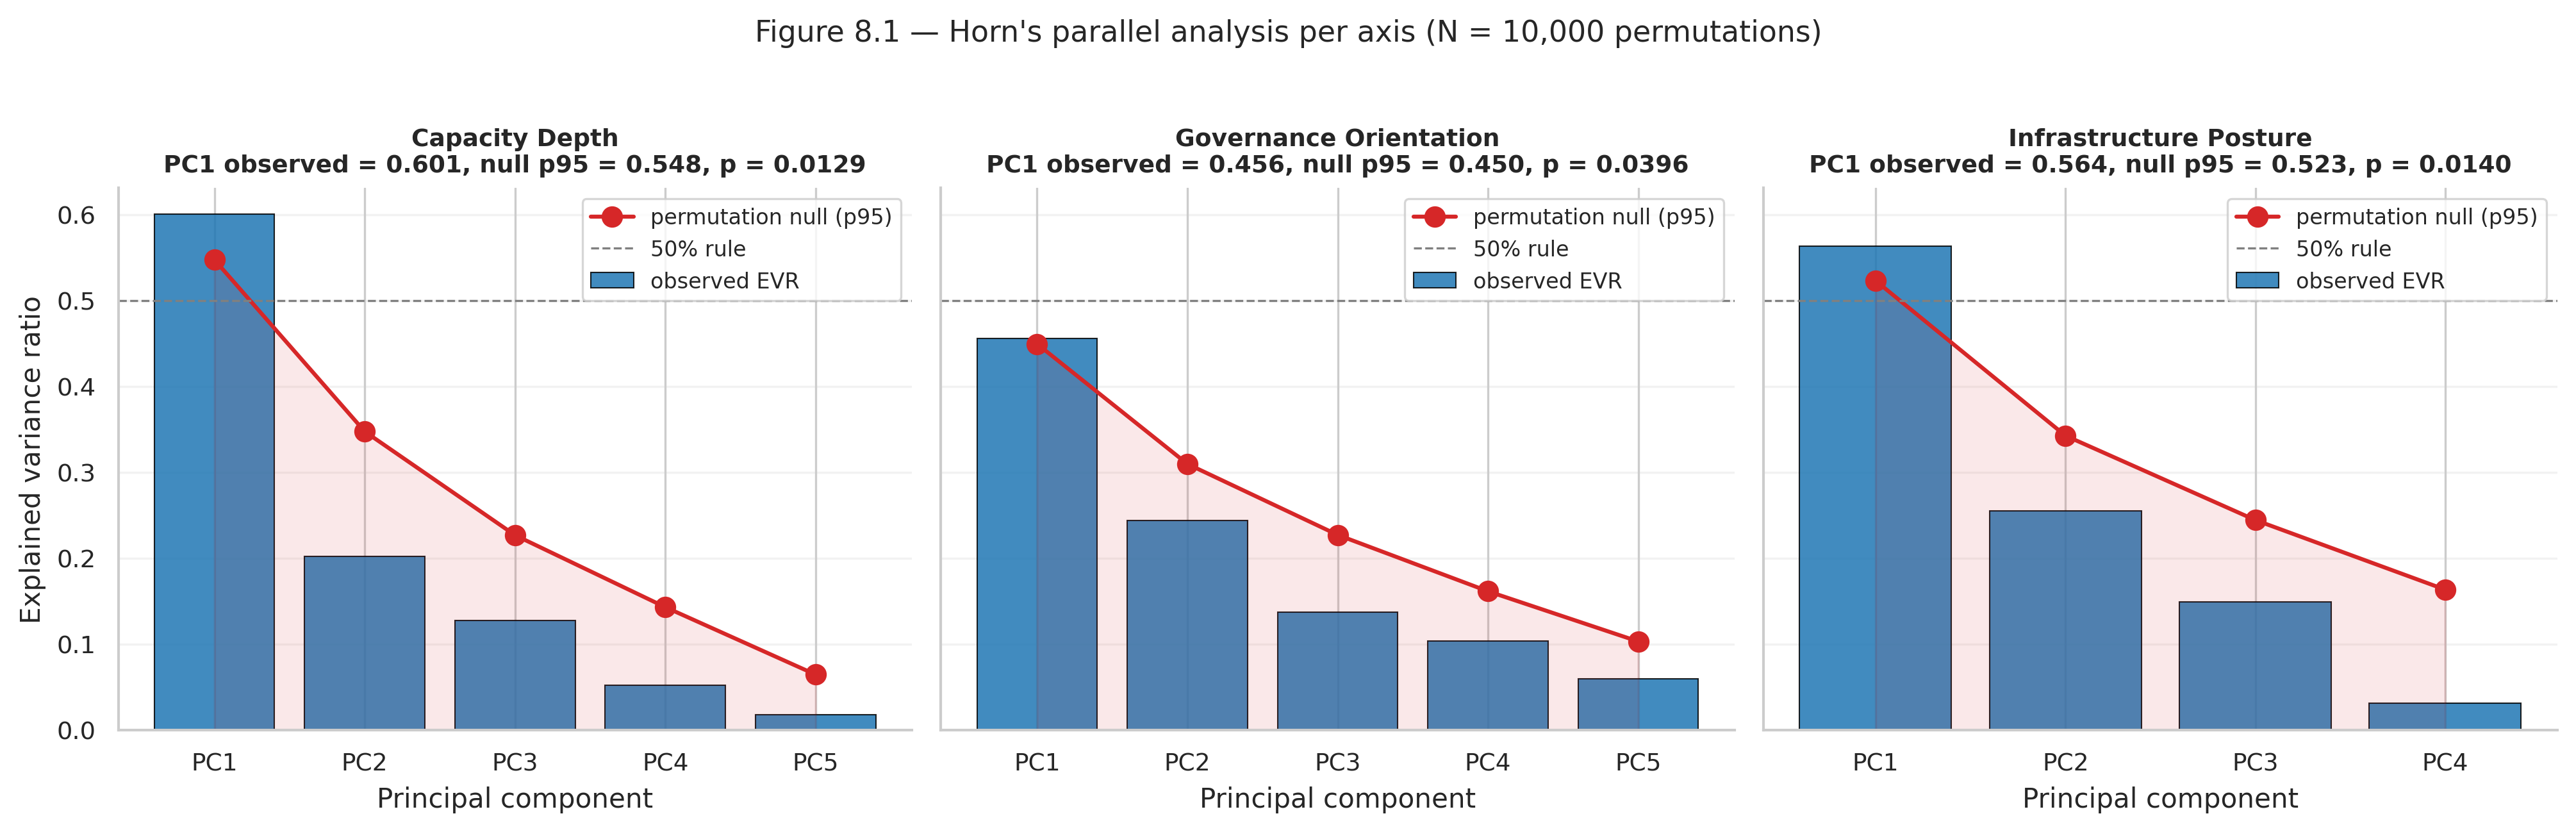
\includegraphics[width=0.97\textwidth]{figures/fig8_1_parallel_analysis.png}
\caption{Horn's parallel analysis per axis ($10{,}000$ permutations). Bars: observed explained-variance ratio per component; red line: $95$th-percentile permutation null; dashed grey: the $50\%$ heuristic. The first component clears the null for governance and infrastructure; capacity is untestable (fit on $n=8$ complete cases, below the ten-case testability floor). Source: \texttt{outputs/parallel\_analysis.csv}.}
\label{fig:pa}
\end{figure}

\subsection{Sensitivity, robustness, and inference}
Rank stability is probed with: a $10{,}000$-draw Dirichlet$(\alpha{=}1)$ Monte Carlo over within- and across-axis weights; leave-one-indicator-out (LOO); a $z$-score-versus-min--max normalisation swap; a bibliographic-classifier swap (broad-AI versus narrow-ML OpenAlex concept for C3); an $\varepsilon$-grid; a C5-axis-reassignment check; and an analyst-coded judgment-collapse check. All rank correlations are reported with Bonett--Wright \citep{bonett2000sample} Fisher-$z$ $95\%$ confidence intervals, whose standard error
\begin{equation}
\mathrm{SE} = \sqrt{\frac{1 + \rho^2/2}{n-3}}
\end{equation}
is the variance-stabilised form appropriate for Spearman's $\rho$ (wider than the naive Pearson $1/\sqrt{n-3}$). A second, \emph{joint} Monte Carlo perturbs the imputed cells alongside the weights---stage-1 axis-mean cells by the country's observed within-axis $z$-dispersion, and stage-2/MNAR cells by $N(0,\sigma_2)$ with $\sigma_2\in\{0.5,1.0\}$---while holding every \emph{observed} value fixed, yielding per-country credible rank intervals and tier-membership probabilities (Section~\ref{sec:results}, Figure~\ref{fig:rankunc}). Concurrent validity is assessed against an independent external index (Section~\ref{subsec:extval}).

\paragraph{Country-influence and weighting-free checks.} Two further checks target the small-$n$ leverage and weight-dependence concerns head-on. A leave-one-\emph{country}-out jackknife \citep{quenouille1949approximate,tukey1958bias} drops each of the fourteen jurisdictions in turn, re-normalises the remaining thirteen (z-scores are sample-relative), and recomputes both the ranking and the $k$-means typology ($k=3$ held fixed to isolate the country-drop effect from model selection), quantifying how much any single country drives the order (Spearman $\rho$ with Bonett--Wright CI on the retained thirteen) and the partition (adjusted Rand index against the full typology). Separately, a \emph{weighting-free} consensus ranking treats each of the fourteen indicators as one equal ballot and aggregates the fourteen ballots with no cardinal weights---neither within- nor across-axis---via the Borda count \citep{borda1781memoire} and the exact Kemeny--Young median ranking \citep{kemeny1959mathematics,young1988optimal}, the order minimising total Kendall-$\tau$ disagreement with the ballots, solved as a mixed-integer programme over the fourteen alternatives. If the headline survives an aggregation that removes the weighting step entirely, the ordering is a property of the data rather than of the weights.

\subsection{Typology and interpretability}
Country archetypes are obtained by $k$-means with a silhouette-selected $k$ \citep{rousseeuw1987silhouettes}, cross-checked against hierarchical clustering (adjusted Rand index, \citealp{hubert1985ari}) and a multidimensional-scaling embedding \citep{kruskal1964mds}. Per-indicator contributions to the headline composite are decomposed exactly by enumerating all $2^{14}$ Shapley \citep{shapley1953value} coalitions, complemented by permutation feature importance and, over the same coalition set, exact second-order Shapley \emph{interaction} indices \citep{grabisch1999interaction} that quantify pairwise indicator redundancy (Appendix~\ref{app:interp}, Figure~\ref{fig:shapint}). Internal consistency, clustering, and MDS use \texttt{scikit-learn} \citep{pedregosa2011scikit}; the stack also includes NumPy \citep{harris2020numpy}, pandas \citep{mckinney2010pandas}, SciPy \citep{virtanen2020scipy}, Matplotlib \citep{hunter2007matplotlib}, and seaborn \citep{waskom2021seaborn}.

% ============================================================
\section{Results}\label{sec:results}
% ============================================================
\subsection{Headline ranking}
Table~\ref{tab:headline} reports the composite under all three schemes. Under the literature scheme South Korea ($2.238$) and the United Kingdom ($2.178$) co-lead---Korea ranks first under the equal and literature schemes, the UK first under PCA---and India ($0.103$) and Taiwan ($0.060$) trail. The top-five set $\{$UK, Korea, France, EU, Japan$\}$ is identical across all three schemes; the bottom-three set contains $\{$India, Taiwan$\}$ under every scheme, with the third slot Israel under the literature scheme and Saudi Arabia under the equal and PCA schemes. Figure~\ref{fig:typology} positions the countries on the capacity $\times$ infrastructure plane, colour-coded by archetype and shape-coded by AISI Network membership.

\begin{table}[t]
\centering
\caption{Headline composite scores under the three weighting schemes, ordered by the literature scheme. The top-five set is invariant across schemes. Source: \texttt{outputs/index\_baseline.csv}.}
\label{tab:headline}
\small
\begin{tabular}{@{}rlccc@{}}
\toprule
\textbf{Rank} & \textbf{Country} & \textbf{Equal} & \textbf{PCA} & \textbf{Literature} \\
\midrule
1  & South Korea           & 2.086 & 2.365 & 2.238 \\
2  & United Kingdom        & 2.083 & 2.420 & 2.178 \\
3  & France                & 1.769 & 2.227 & 1.928 \\
4  & Japan                 & 1.701 & 2.055 & 1.764 \\
5  & European Union        & 1.750 & 2.299 & 1.750 \\
6  & Singapore             & 1.324 & 1.622 & 1.731 \\
7  & Germany               & 1.339 & 1.820 & 1.411 \\
8  & Canada                & 1.381 & 2.027 & 1.383 \\
9  & Sweden                & 0.883 & 1.275 & 1.049 \\
10 & United Arab Emirates  & 0.314 & 0.382 & 0.885 \\
11 & Saudi Arabia          & 0.106 & 0.113 & 0.793 \\
12 & Israel                & 0.329 & 0.888 & 0.132 \\
13 & India                 & 0.077 & 0.098 & 0.103 \\
14 & Taiwan                & 0.077 & 0.117 & 0.060 \\
\bottomrule
\end{tabular}
\end{table}

\begin{figure}[t]
\centering
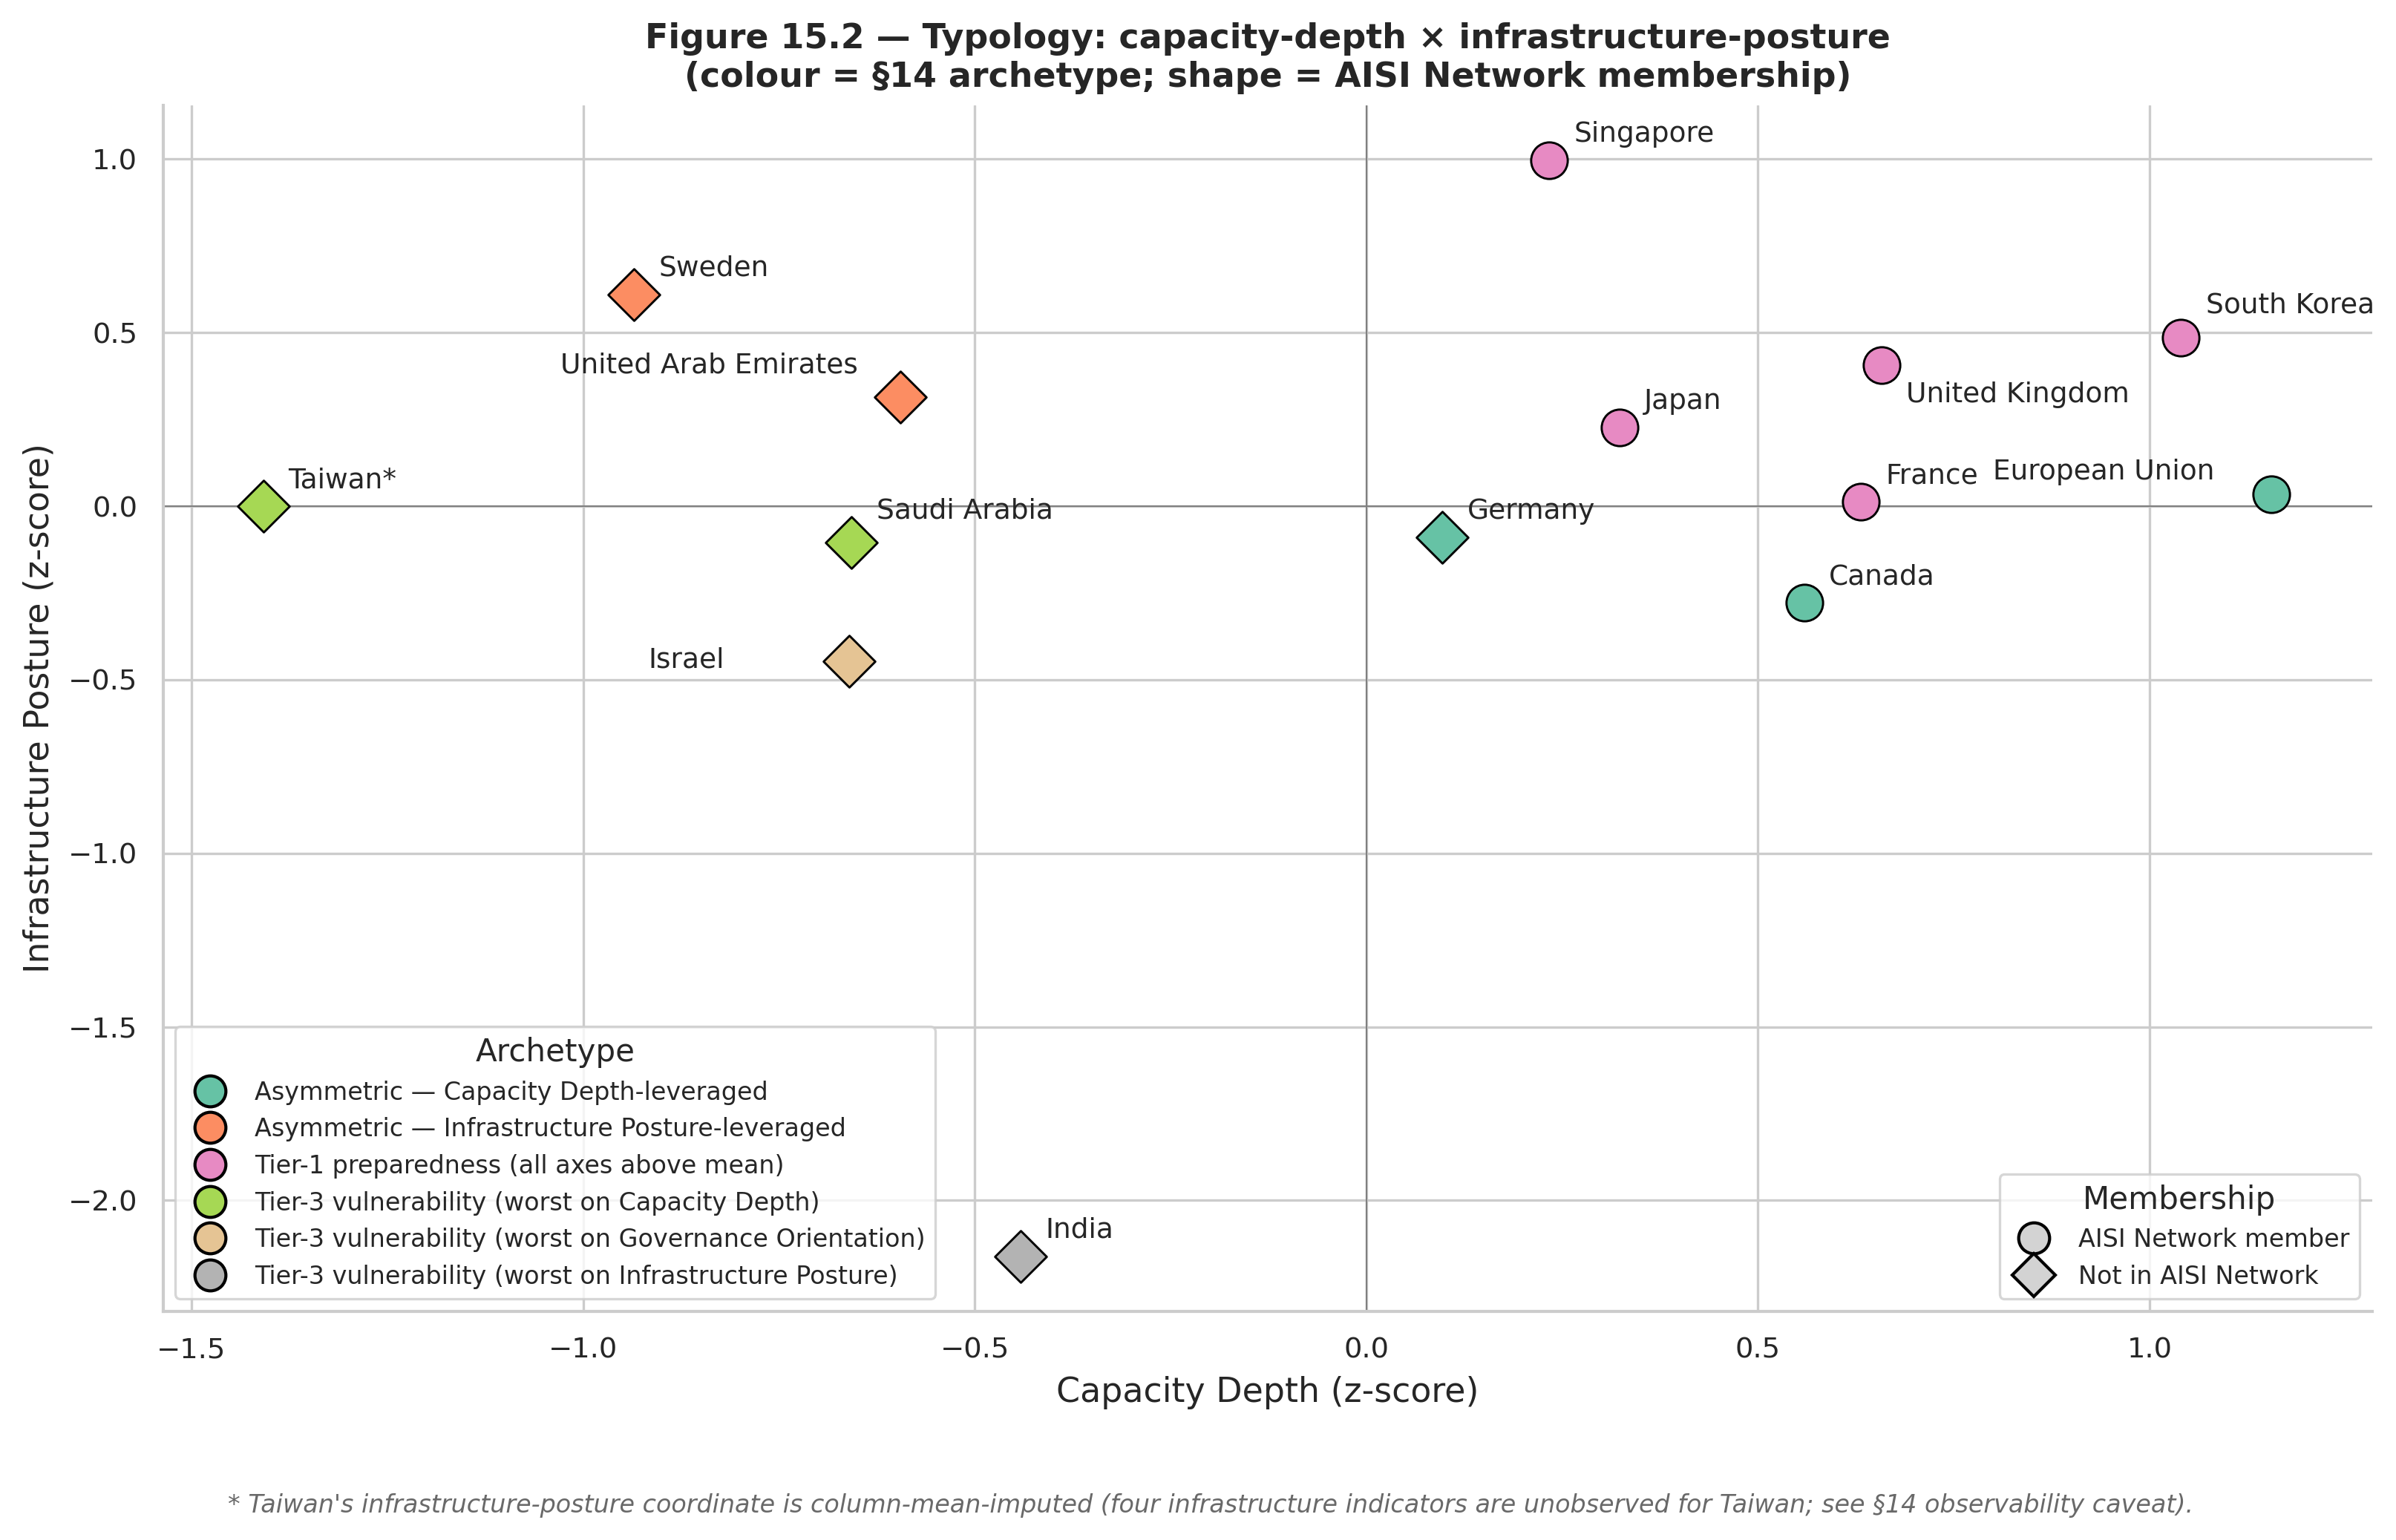
\includegraphics[width=0.9\textwidth]{figures/fig15_2_typology.png}
\caption{Country positions on Capacity Depth $\times$ Infrastructure Posture ($z$-scores). Colour encodes the per-country archetype derived from each country's own axis profile (Tier-1; two Asymmetric variants; three Tier-3 variants by worst axis); marker shape encodes AISI Network membership. Taiwan's infrastructure coordinate is column-mean-imputed. Source: \texttt{outputs/typology.csv}.}
\label{fig:typology}
\end{figure}

\subsection{Robustness}
Under the Bonett--Wright standard error, the equal-vs-PCA, equal-vs-literature, and normalisation perturbations all clear the $0.70$ robustness floor with comfortable margins, and their CI lower bounds ($0.911$, $0.861$, and $0.861$) also clear the stricter $0.85$ bar (Table~\ref{tab:robust}, Figure~\ref{fig:forest}). Only the bibliographic-classifier check ($\rho=0.960$, CI lower bound $0.845$) sits just below the $0.85$ bar imposed on the classifier (a core measurement choice rather than a downstream weight perturbation), while still clearing the $0.70$ floor. The Monte Carlo rank distributions (Appendix Figure~\ref{fig:rankdist}) show the United Kingdom and South Korea co-leading at a median rank of~2 and the $\{$France, Japan, EU$\}$ block sharing a median rank of~4.

\begin{table}[t]
\centering
\caption{Robustness of the headline ranking. Spearman $\rho$ against the literature ranking with Bonett--Wright Fisher-$z$ $95\%$ CIs ($n=14$). Source: \texttt{outputs/robustness\_summary\_with\_ci.csv}.}
\label{tab:robust}
\small
\begin{tabular}{@{}lcccc@{}}
\toprule
\textbf{Perturbation} & \textbf{$\rho$} & \textbf{Threshold} & \textbf{95\% CI} & \textbf{Verdict} \\
\midrule
Weighting: equal vs PCA            & 0.978 & 0.70 & $[0.911,\,0.995]$ & clears \\
Weighting: equal vs literature     & 0.965 & 0.70 & $[0.861,\,0.992]$ & clears \\
Normalisation: $z$ vs min--max     & 0.965 & 0.70 & $[0.861,\,0.992]$ & clears \\
Classifier: AI-broad vs ML-narrow  & 0.960 & 0.85 & $[0.845,\,0.990]$ & borderline \\
\bottomrule
\end{tabular}
\end{table}

\begin{figure}[t]
\centering
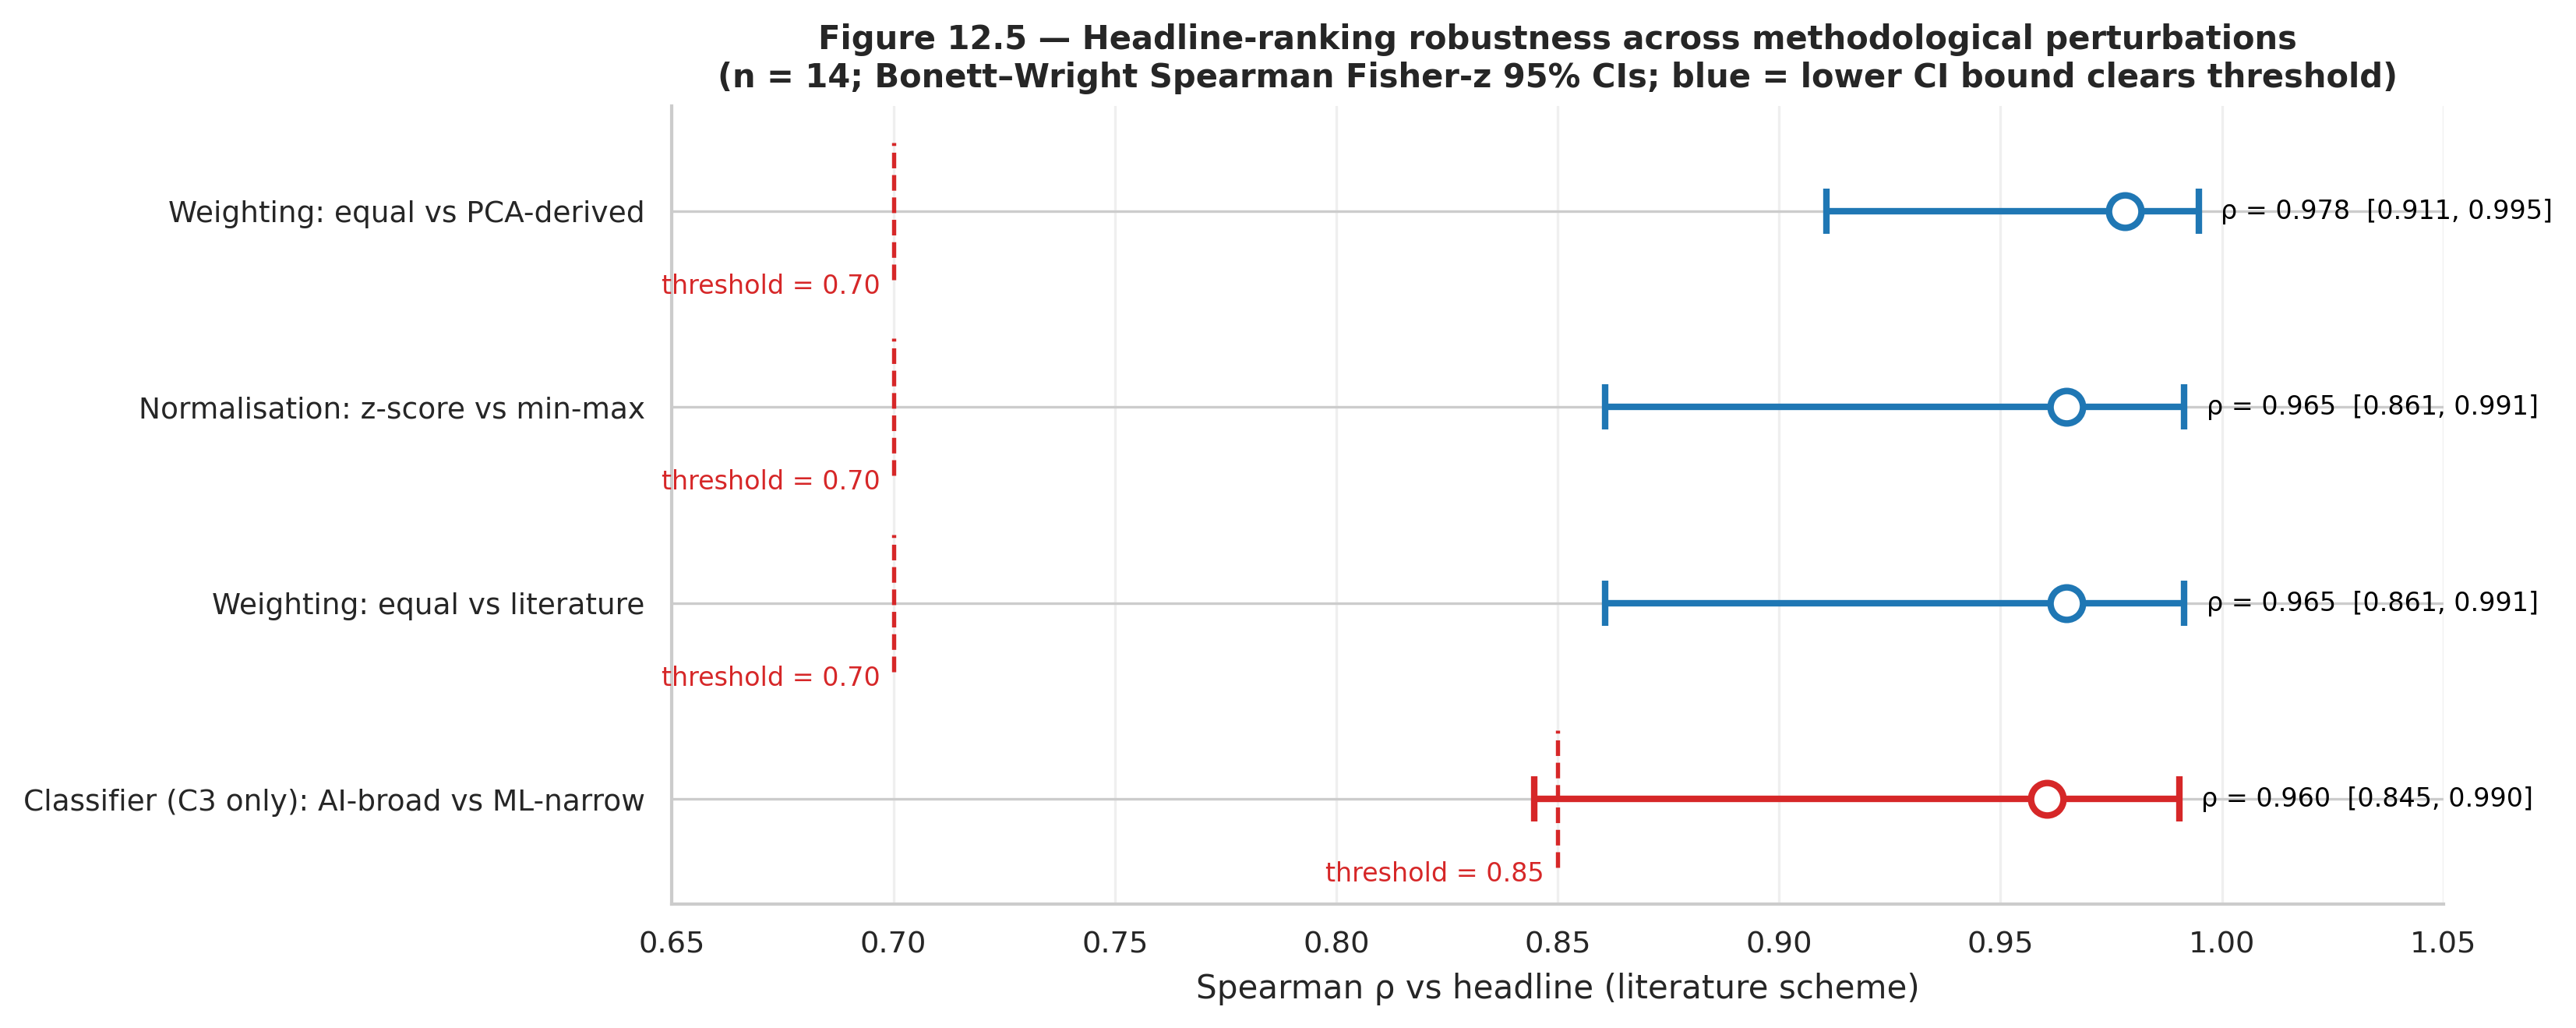
\includegraphics[width=0.92\textwidth]{figures/fig12_5_robustness_forest.png}
\caption{Robustness forest plot: Spearman $\rho$ point estimates with Bonett--Wright Fisher-$z$ $95\%$ CIs against each perturbation's pass threshold (dashed). The equal-vs-PCA, equal-vs-literature, and normalisation checks clear $0.70$ with wide margins (all three CI lower bounds also clear $0.85$); only the classifier check is borderline against the stricter $0.85$ bar applied to it. Source: \texttt{outputs/robustness\_summary\_with\_ci.csv}.}
\label{fig:forest}
\end{figure}

\paragraph{Rank uncertainty.} The joint Monte Carlo---perturbing weights \emph{and} imputed cells while holding observed values fixed---attaches an uncertainty band to every position. Under the most conservative setting ($\sigma_2=1.0$), the United Kingdom and South Korea each sit in the top five in about $98\%$ of draws (co-leading at a median rank of~2); the bottom tier is weaker (India and Taiwan in the bottom three in $76\%$ and $61\%$ of draws). The added imputation noise widens the credible intervals only marginally over the weight-only Monte Carlo (Figure~\ref{fig:rankunc}), confirming that the headline ordering is not an artefact of the fixed imputed values---the cells the pipeline had to fill do not drive the ranking. The middle of the table is where the bands overlap most, consistent with the single-slot instability behind H6's partial verdict.

\begin{figure}[t]
\centering

\includegraphics[width=0.86\textwidth]{figures/fig12_9_rank_uncertainty.png}
\caption{Joint rank-uncertainty: $95\%$ credible rank intervals from $10{,}000$ draws, weight-only (Section~\ref{sec:methods}, §12.1) versus joint weights-plus-imputed-cell perturbation ($\sigma_2=1.0$); red markers are the headline ranks. Observed Tier-1 values are held fixed; only imputed cells are resampled. Source: \texttt{outputs/rank\_uncertainty.csv}.}
\label{fig:rankunc}
\end{figure}

\paragraph{Country influence and weighting-free consensus.} Two further checks (Section~\ref{sec:methods}) confirm the ordering is neither a single-country artefact nor a weighting artefact. The leave-one-\emph{country}-out jackknife shows that dropping any one jurisdiction shifts the retained thirteen by at most three rank positions (worst case: dropping India or Taiwan), the retained-order Spearman $\rho$ never falls below $0.945$, and the $k$-means typology is identical (ARI $=1.0$) for twelve of the fourteen drops---dipping only when India, the singleton archetype, is removed (ARI $=0.61$). The weighting-free consensus is equally reassuring: aggregating the fourteen indicator ballots with \emph{no} cardinal weights reproduces the literature ordering under both the Borda count (Spearman $\rho=0.979$, $95\%$ CI $[0.915,\,0.995]$) and the exact Kemeny--Young median ranking ($\rho=0.930$, $[0.739,\,0.982]$). South Korea is first under both and the top-five and bottom-three sets are preserved under Borda; the only consequential disagreement is that the Kemeny median elevates Germany into the fifth slot and demotes Japan to seventh---a weight-independent reminder that the 3--5 block is the table's soft region (Appendix Figures~\ref{fig:loocountry} and~\ref{fig:rankagg}).

\subsection{Pre-registered hypotheses}
Table~\ref{tab:hyp} records the six hypotheses, their numeric pass criteria, and their mechanically resolved verdicts. Two are fully supported (H3, H5) and four are partially supported with named caveats (H1, H2, H4, H6). The partial verdicts surface specific methodological caveats---a near-collinear pair across two axes (C5$\times$G1, Pearson $r=0.965$), governance multidimensionality, one borderline robustness check (the bibliographic classifier), and a weight-sensitive bottom tier---rather than a wholesale framework failure. The C5$\times$G1 collinearity is the largest of only five cross-axis indicator pairs at $|r|\geq0.7$ (of 65 pairs).

\begin{table}[t]
\centering
\caption{The six pre-registered hypotheses (criteria fixed before estimation) and their mechanically resolved verdicts.}
\label{tab:hyp}
\footnotesize
\begin{tabularx}{\textwidth}{@{}l Y l Y@{}}
\toprule
\textbf{ID} & \textbf{Hypothesis} & \textbf{Verdict} & \textbf{Evidence} \\
\midrule
H1 & The three axes are empirically separable. & Partial & $5$ of $65$ cross-axis pairs at $|r|\geq0.7$; C5$\times$G1 ($r=0.965$) is the largest contributor. \\
H2 & Each axis carries a one-dimensional signal. & Partial & Infrastructure $p=0.014$, governance $p=0.040$ (both significant); capacity untestable at $n=8$; governance PC1 explains $45.6\%$. \\
H3 & The 14 powers do not cluster homogeneously. & Supported & Silhouette $0.426$ at $k=3$; ARI $=1.0$ vs complete and average linkage ($0.727$ vs Ward); MDS distance-rank $\rho=0.910$. \\
H4 & The ranking is robust to perturbation. & Partial & Equal-vs-PCA, equal-vs-literature, and normalisation clear the $0.85$ bar (CI lower bounds $0.911$/$0.861$/$0.861$); only the classifier (CI lower bound $0.845$) sits below it. \\
H5 & The top-5 is not driven by any one coded indicator. & Supported & Top-5 set unchanged dropping either G1 or C5; judgment-collapse min $\rho=0.996$, max single-country shift $1$. \\
H6 & Top-5 and bottom-3 tier membership are stable. & Partial & $5/5$ top-5 members in tier in $\geq70\%$ of draws; no bottom-3 member reaches $80\%$, Israel only $50.4\%$, cycling with Saudi Arabia. \\
\bottomrule
\end{tabularx}
\end{table}

\subsection{Vulnerability overlay}
Applying the per-vector weights (Table~\ref{tab:vectorweights}) to the literature axis scores yields per-country preparedness scores on each attack vector (Figure~\ref{fig:vuln}; full ranks in Appendix Table~\ref{tab:vuln}). The United Kingdom and South Korea lead on all three vectors; the lower tier (Israel, Taiwan, India) is least prepared, with vector-specific reordering---India is weakest on cyber and influence operations, Taiwan weakest on CBRN. Per-vector scores are signed $z$-scale quantities (positive $=$ above sample-mean preparedness) and are interpretable only within a vector, not across vectors.

\begin{figure}[t]
\centering
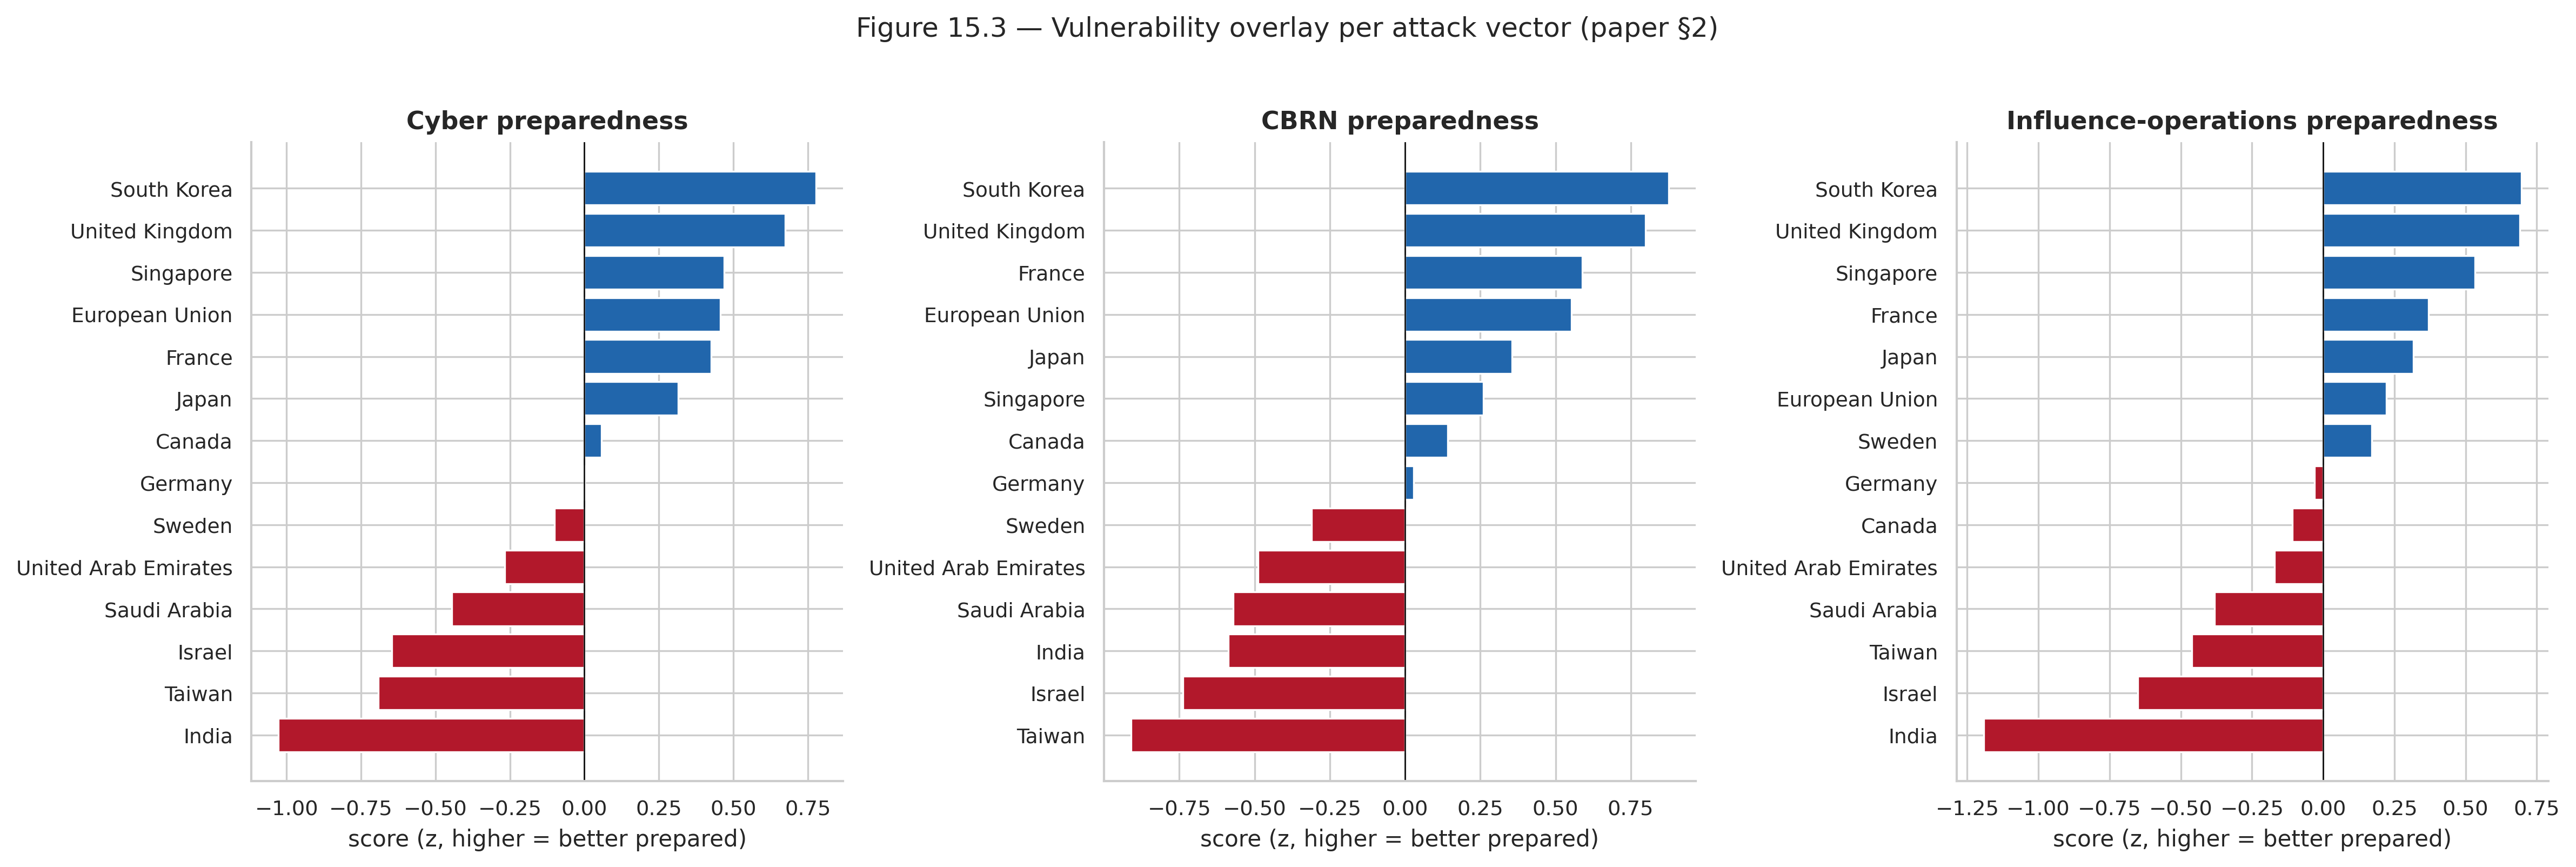
\includegraphics[width=0.97\textwidth]{figures/fig15_3_vulnerability.png}
\caption{Per-vector preparedness (paper $\S$2): cyber, CBRN, and influence operations. Each panel is sorted independently; bars are signed $z$-scale scores (higher $=$ better prepared). Source: \texttt{outputs/vulnerability\_overlay.csv}.}
\label{fig:vuln}
\end{figure}

\subsection{Counterfactual policy leverage}
To operationalise the paper's $\S$4 claim that tractability depends on axis position, we recompute the composite under four direct policy actions per country (e.g.\ joining the AISI Network, publishing a safety-provisioned AI strategy, joining the Australia Group). Figure~\ref{fig:cf} reports the composite change; the highest-leverage action differs by country and by starting position. For example, with Singapore selected, joining the Australia Group raises its composite from $1.731$ to $1.841$ (rank 6 to 4). For countries at an axis minimum, the geometric-shift artefact can understate the composite change, so an axis-level reading is reported alongside.

\begin{figure}[t]
\centering
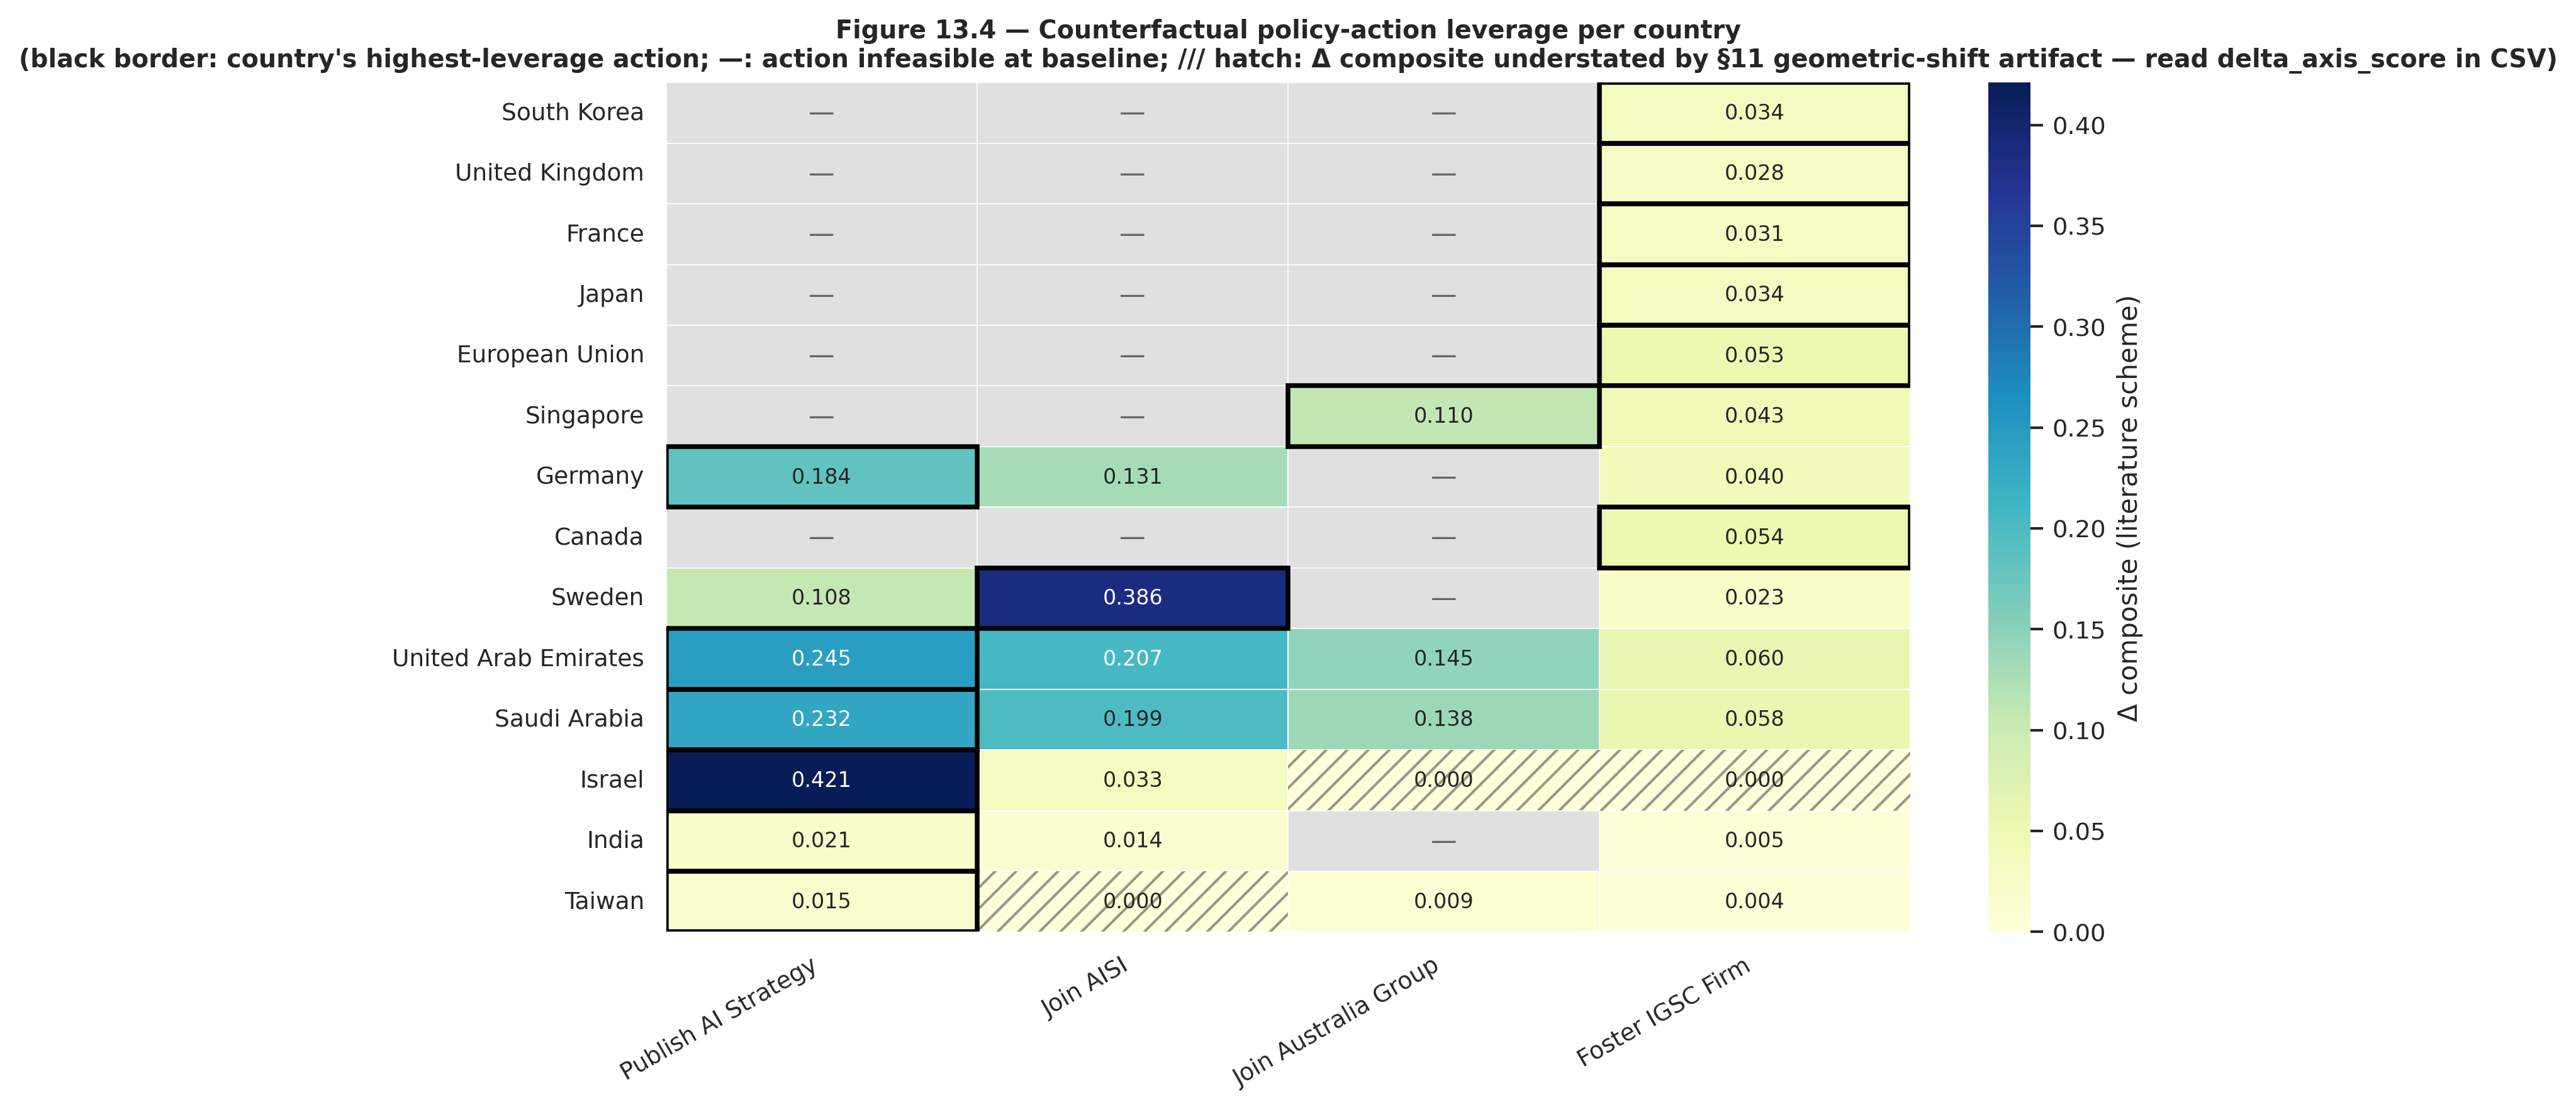
\includegraphics[width=0.95\textwidth]{figures/fig13_4_counterfactual_heatmap.png}
\caption{Counterfactual policy-action leverage per country (composite change under the literature scheme). Black border: the country's highest-leverage action; em-dash: action already satisfied at baseline; hatching: a geometric-shift artefact for which the axis-level change should be read instead. Source: \texttt{outputs/counterfactual\_scenarios.csv}.}
\label{fig:cf}
\end{figure}

\subsection{Minimal-action-set optimisation}\label{subsec:mas}
The counterfactuals above move one lever at a time; the working paper's $\S$4 \emph{tractability} claim is sharper---which improvements are \emph{reachable}, and at what effort. Enumerating the full $2^4 = 16$ action space per country (counting only \emph{effective} actions, so a country already in the AISI Network pays nothing to ``join'' it), we identify each below-top country's \emph{minimal action set}: the fewest effective actions that lift it into the next composite-rank tier (bottom-3 $\to$ middle $\to$ top-5; Figure~\ref{fig:mas}). Tractability is starkly heterogeneous. Only three of the nine below-top jurisdictions can cross into the next tier through these four levers at all: Singapore needs a single action (join the Australia Group: rank 6 $\to$ 4), Israel a single action (publish a safety-provisioned AI strategy: rank 12 $\to$ 10), and Germany three (join the AISI Network, publish a strategy, and foster an IGSC firm: rank 7 $\to$ 4). The remaining six---Canada, Sweden, the UAE, Saudi Arabia, India, and Taiwan---cannot reach the next tier through these governance/capacity levers alone; India and Taiwan in particular are held down by infrastructure and capacity deficits the four actions do not address. This is an explicit, per-country statement of \emph{where} preparedness is cheaply tractable and where it is not---exactly the question $\S$4 raises. Cost here is action count; a weighted-cost variant is a drop-in substitution.

\begin{figure}[t]
\centering

\includegraphics[width=0.9\textwidth]{figures/fig13_7_minimal_action_sets.png}
\caption{Minimal action set per below-top country: the fewest effective actions (blue) that reach the next composite tier; rows marked unreachable cannot cross with the four levers. Unit cost; reuses the §13.4 recompute. Source: \texttt{outputs/minimal\_action\_sets.csv}.}
\label{fig:mas}
\end{figure}

\subsection{Causal-interpretation boundary}\label{subsec:causal}
The counterfactuals (\S\ref{subsec:mas} and Figure~\ref{fig:cf}) are \emph{mechanical recomputations of the index} under a hypothetical indicator change---they answer ``if indicator $X$ took value $x'$, the composite would move by $\Delta$''---not estimates of the causal effect of a policy on real-world preparedness, and we do not present them as such. Reading a counterfactual $\Delta$ causally would require, in the language of Pearl's do-calculus \citep{pearl2009causal} and the potential-outcomes framework \citep{hernan2020causal}, a well-defined intervention, no unmeasured confounding, no interference between units, temporal precedence, and structural stability---none of which a single cross-sectional snapshot of $n = 14$ jurisdictions satisfies: AISI membership and strategy comprehensiveness co-vary with latent state capacity (the C5$\times$G1 $r = 0.965$ signal), one country's action shifts others' \emph{relative} ranks, and cause and outcome are observed simultaneously (Figure~\ref{fig:dag}; the full assumptions ledger is in \texttt{outputs/causal\_assumptions.csv}). The counterfactuals are therefore index-structural sensitivity probes and tractability illustrations, consistent with $\S$4's qualitative framing, while the paper's $\S$3 trigger-event/causal claims remain explicitly out of scope pending country-year incident data (Section~\ref{sec:limits}).

\begin{figure}[t]
\centering
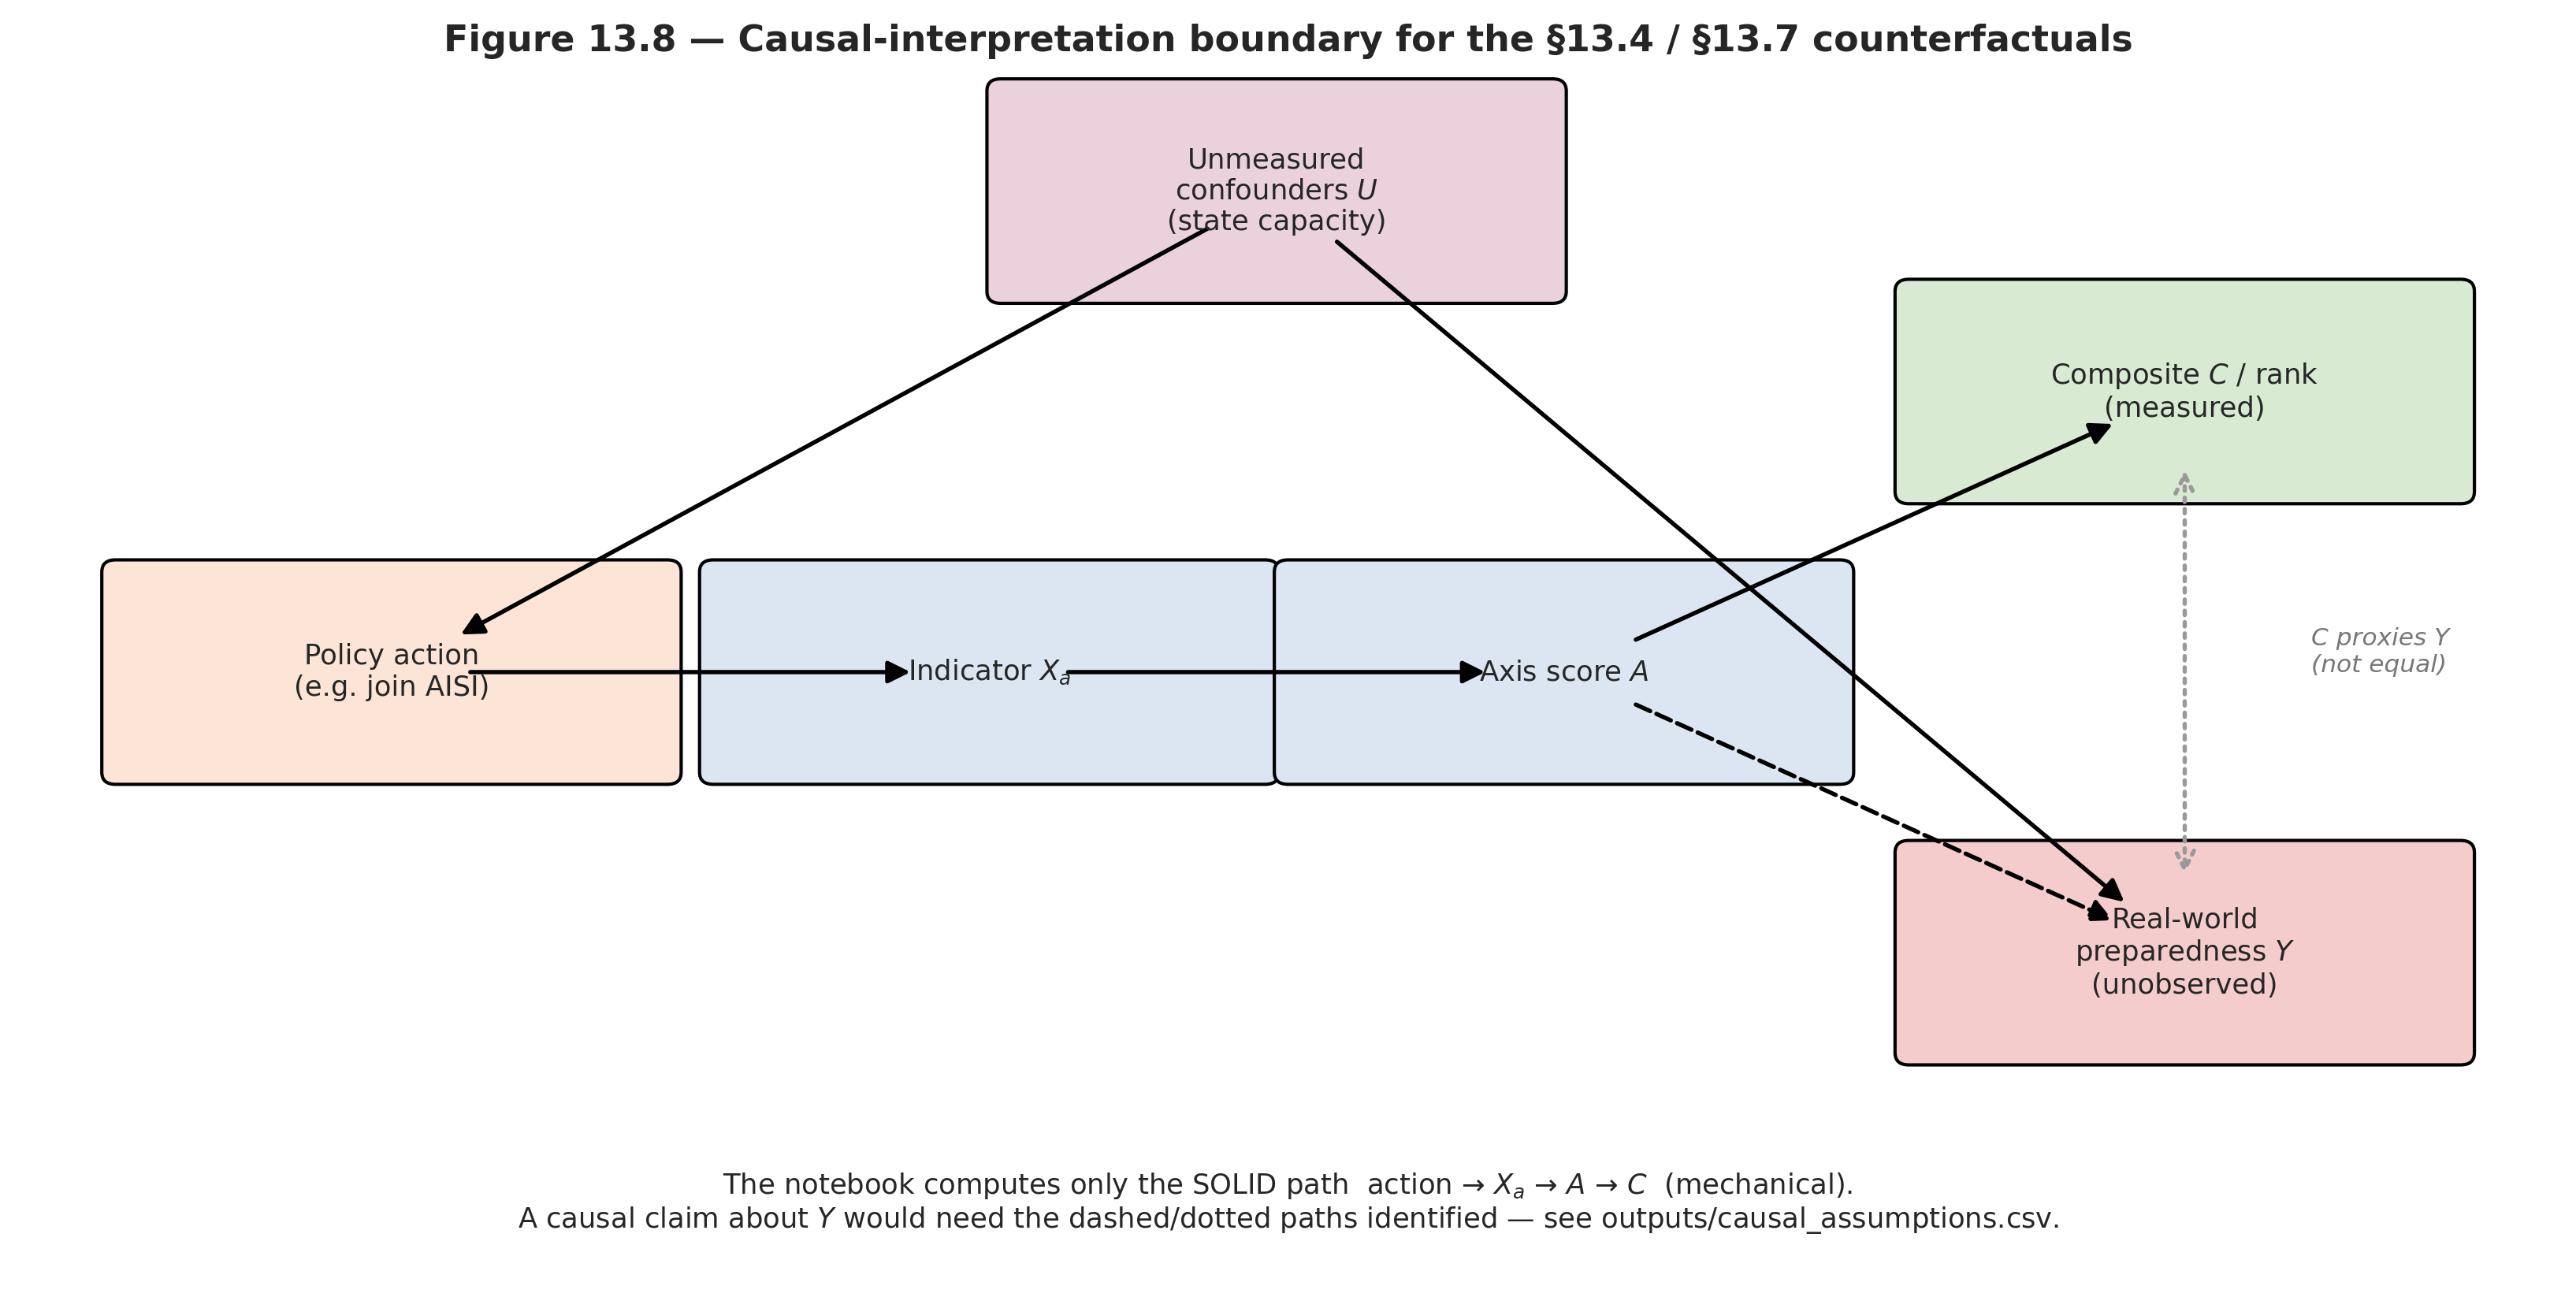
\includegraphics[width=0.85\textwidth]{figures/fig13_8_causal_dag.png}
\caption{Causal-interpretation boundary for the counterfactuals. The index computes only the solid path (action $\to X_a \to A \to$ composite $C$); a causal claim about real-world preparedness $Y$ would need the dashed/dotted paths identified, which an $n = 14$ cross-section cannot do. Source: \texttt{outputs/causal\_assumptions.csv}.}
\label{fig:dag}
\end{figure}

\subsection{Typology}
The silhouette-selected $k=3$ $k$-means partition separates a Tier-1/asymmetric-developed group, a mid group, and India as a singleton; the partition is identical to complete- and average-linkage hierarchical clustering (ARI $=1.0$) and close to Ward (ARI $=0.727$). The MDS embedding (Figure~\ref{fig:mds}) preserves the pairwise-distance rank at $\rho=0.910$ and visually separates the archetypes.

\begin{figure}[t]
\centering

\includegraphics[width=0.86\textwidth]{figures/fig14_3_mds_embedding.png}
\caption{Multidimensional-scaling embedding of the 14 jurisdictions in the full fourteen-indicator space (distance-rank $\rho=0.910$). Colour: archetype; marker shape: AISI Network membership. Source: \texttt{outputs/mds\_coordinates.csv}.}
\label{fig:mds}
\end{figure}

% ============================================================
\section{Discussion: how the index supports the working paper}\label{sec:discussion}
% ============================================================
The index supplies the empirical layer the working paper asserts but does not provide.

\paragraph{It grounds the $\S$1 premise.} The paper claims the fourteen middle powers ``differ along three axes.'' H3 confirms this empirically: the countries do not cluster homogeneously (silhouette $0.426$; a $k$-means partition identical to complete- and average-linkage clustering, ARI $=1.0$, and close to Ward, ARI $=0.727$), and the typology identifies coherent archetypes---Tier-1 (UK, Korea, France, Japan, Singapore), capacity-leveraged (EU, Canada, Germany), infrastructure-leveraged (Sweden, UAE), and a Tier-3 vulnerable group (Israel, Saudi Arabia, India, Taiwan).

\paragraph{It identifies the most-exposed tier.} The paper argues that lower-capacity middle powers face a ``structurally under-addressed vulnerability.'' The index makes that tier concrete and reproducible: India and Taiwan are the two lowest-ranked composites under all three weighting schemes, and the three least-prepared states on every per-vector overlay are India, Israel, and Taiwan (in vector-specific order); the third bottom-tier composite slot cycles between Israel and Saudi Arabia (the single-slot instability behind H6's partial verdict). This illustrates---rather than merely asserts---which states the paper's argument most urgently concerns.

\paragraph{It quantifies $\S$4 tractability.} The paper repeats that ``tractability depends on a country's position within the three axes'' without specifying any action's leverage. The counterfactual scenarios (Figure~\ref{fig:cf}) convert this into a per-country, per-action quantity: the highest-leverage step differs by starting position, exactly as the paper's qualitative argument implies.

\paragraph{Defensibility.} Three design choices keep the study reviewable. First, \emph{bounded scope}: the index operationalises $\S$1--$\S$2 and explicitly declines $\S$3--$\S$4. Second, \emph{census, not sample}: the fourteen jurisdictions are the population the paper names, so the descriptive claims are exact and the small-$n$ multivariate methods are caveated diagnostics rather than load-bearing inference. Third, \emph{transparency}: every weakness is disclosed and bounded by a dedicated sensitivity analysis, and the partial-support verdicts are reported as such.

\subsection{External concurrent validity}\label{subsec:extval}
A composite is only as credible as its agreement with \emph{independent} measures of the same construct. None of M-PAPI's indicators is itself a published readiness score, so the index can be benchmarked against one without circularity. The natural comparator is the Oxford Insights Government AI Readiness Index 2024 \citep{oxfordinsights2024gairi}, an independently constructed index over 188 jurisdictions and 40 indicators that is \emph{not} an input to M-PAPI. Because it scores sovereign states, it covers thirteen of the fourteen middle powers---the EU bloc is the sole exclusion, mirroring the Section~\ref{sec:results} EU-vs-member-state treatment---and Taiwan \emph{is} covered. Across the thirteen, the M-PAPI literature composite and the GAIRI overall score are strongly rank-concordant: Spearman $\rho=0.863$ ($95\%$ CI $[0.521,\,0.966]$, $n=13$; Figure~\ref{fig:extval}). The agreement evidences that M-PAPI tracks a real, externally corroborated readiness gradient rather than an artefact of its own weighting. The divergences are equally informative and expected by construction: Singapore ranks first on GAIRI but sixth on the full M-PAPI ranking (fifth among the thirteen GAIRI-covered jurisdictions, with the EU excluded), and the United Kingdom and Japan rank higher on M-PAPI than on GAIRI---M-PAPI deliberately rewards the CBRN/biosecurity-governance signals (Australia Group membership, IGSC participation, AISI-network presence) that a general-purpose government-readiness index omits, which is precisely the proliferation-specific lens the working paper calls for.

\begin{figure}[t]
\centering
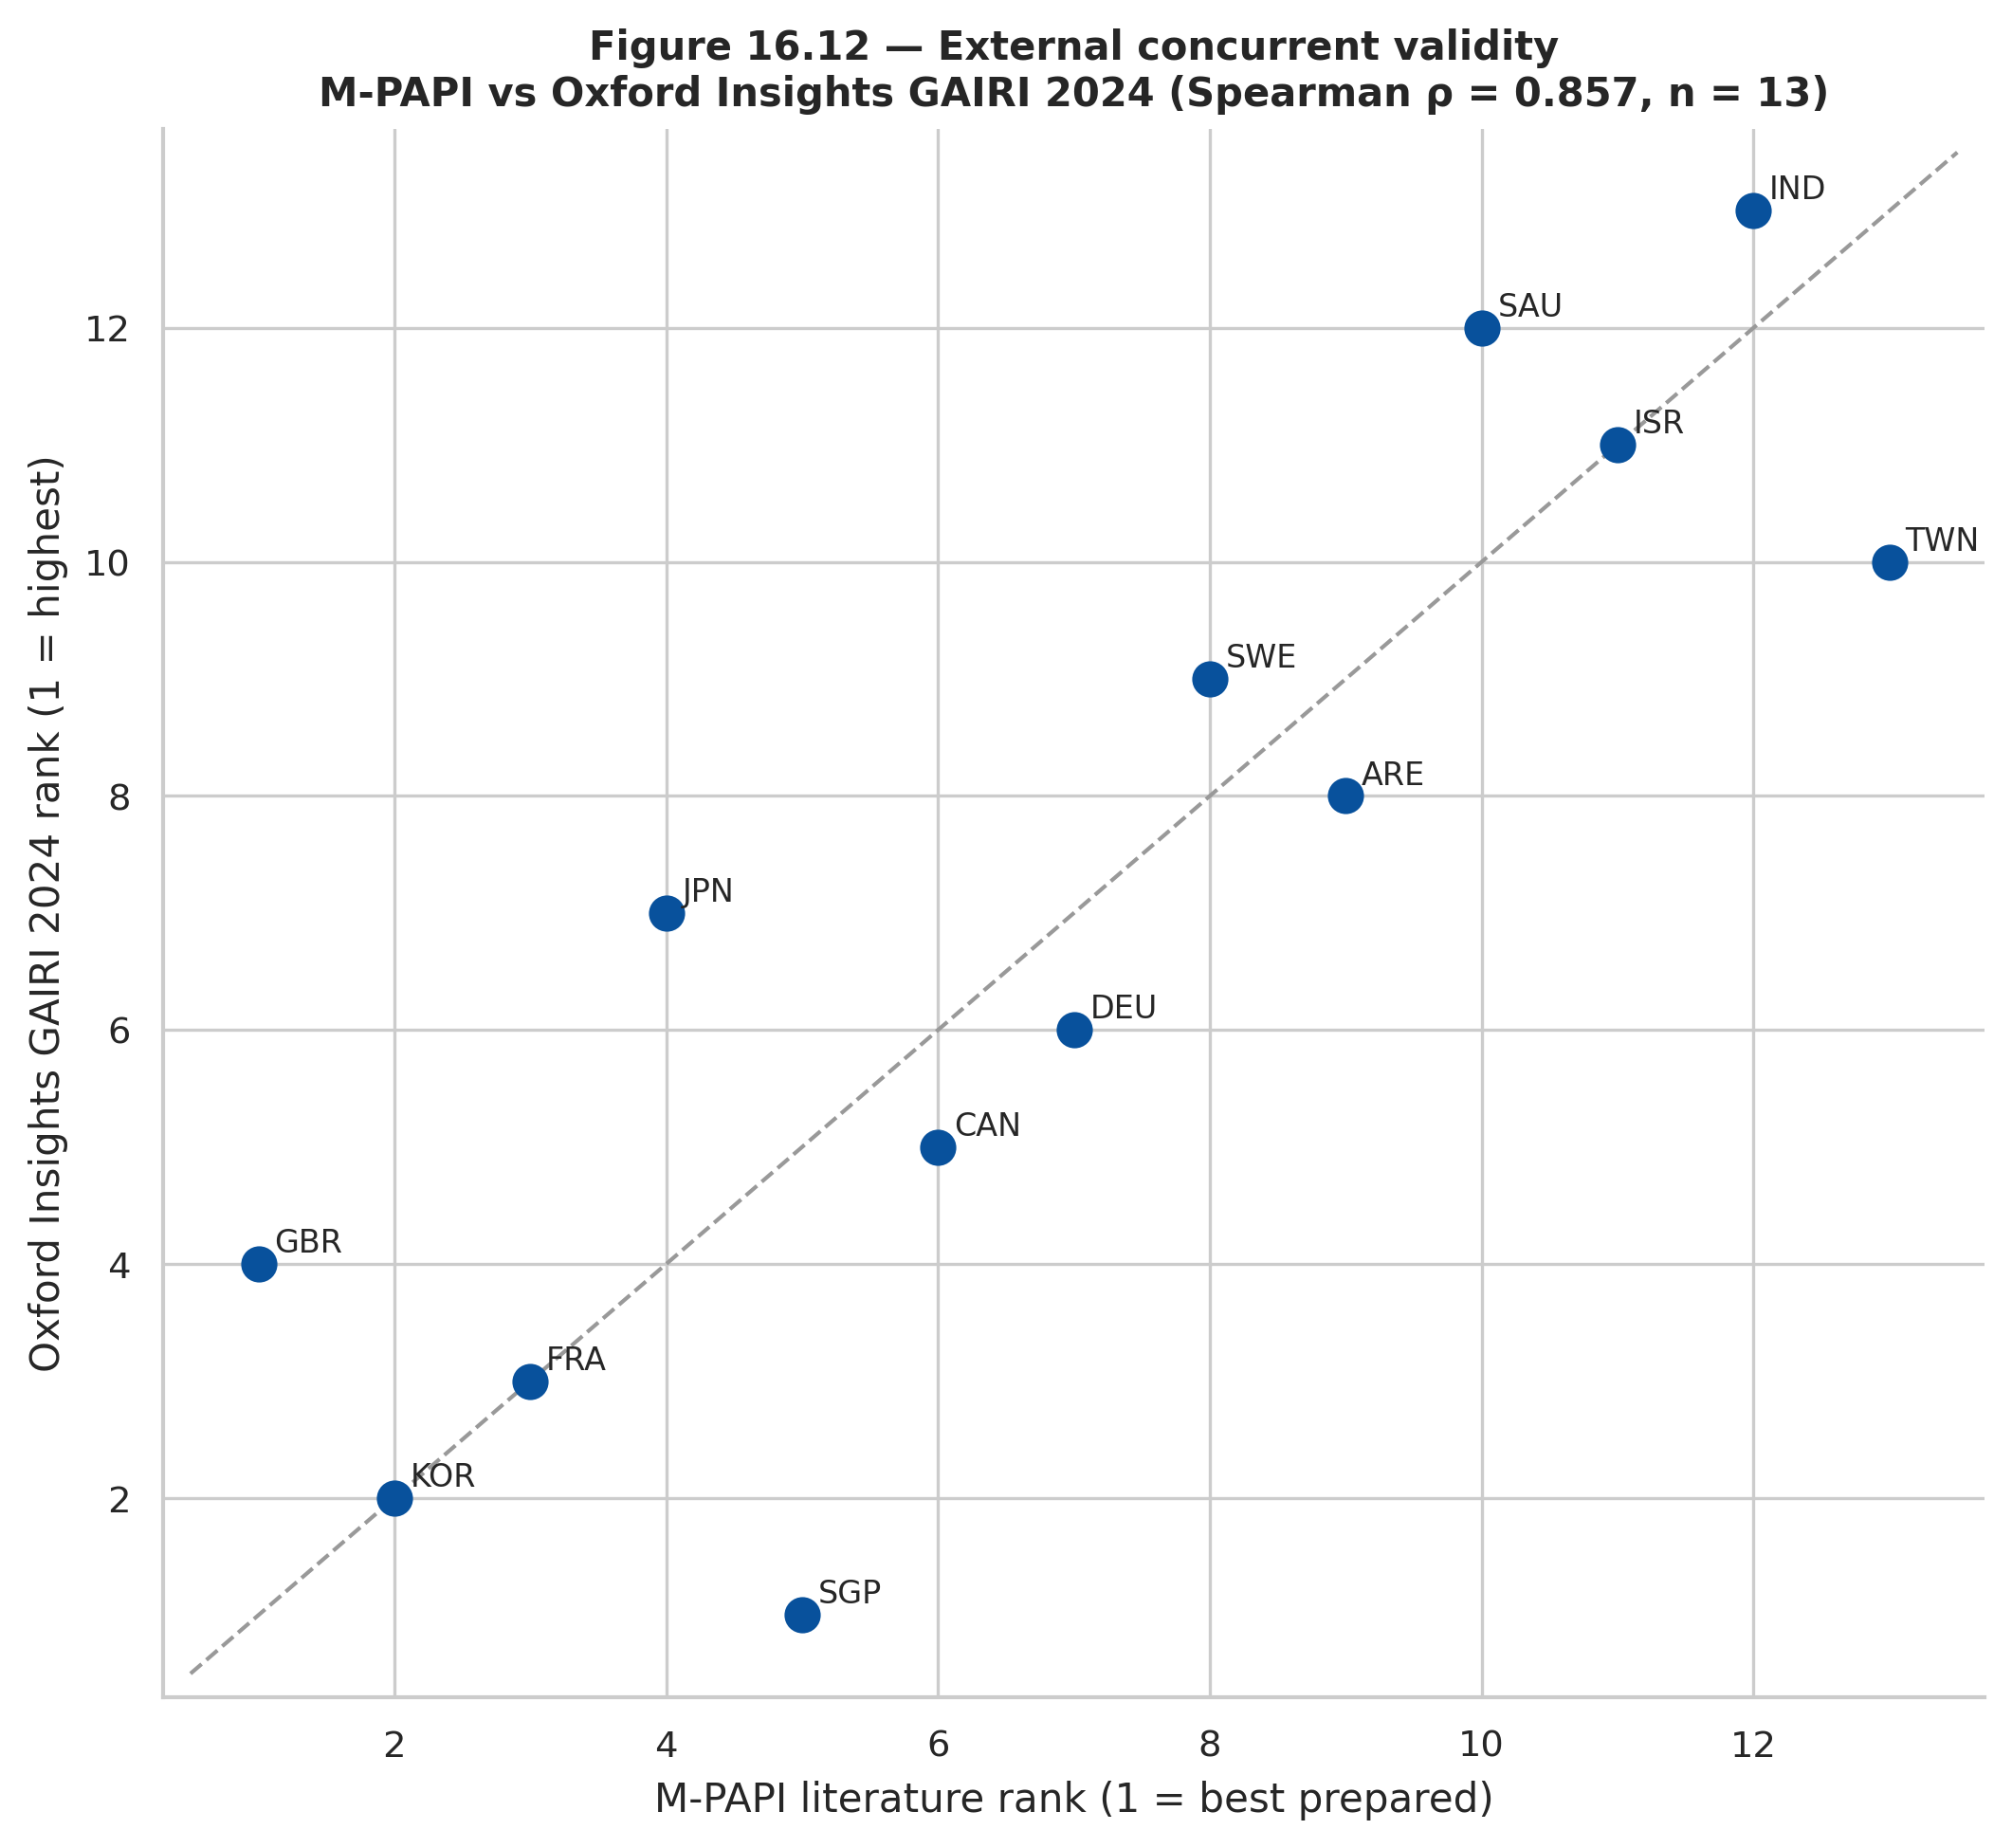
\includegraphics[width=0.62\textwidth]{figures/fig16_12_external_validity.png}
\caption{External concurrent validity: M-PAPI literature rank versus Oxford Insights GAIRI 2024 rank across the thirteen covered jurisdictions (the EU bloc is unscored by GAIRI). Points near the diagonal agree; Spearman $\rho=0.863$. Source: \texttt{outputs/external\_validity.csv}.}
\label{fig:extval}
\end{figure}

% ============================================================
\section{Limitations and threats to validity}\label{sec:limits}
% ============================================================
Following \citet{shadish2002experimental}, we organise residual risks by validity type.

\textbf{Construct validity.} Several indicators are disclosed proxies whose link to the axis label is indirect: ND-GAIN readiness (I5) is a climate-adaptation measure used as an infrastructure-resilience proxy; V-Dem (G3) measures political-system democracy, not AI governance \emph{per se}; the IGSC count (G5) measures industrial biosecurity participation; and secure-server density (I3) increasingly reflects certificate-registration jurisdiction rather than substantive infrastructure. These are the most pressable choices; the defence is that the axes are the paper's, the proxies are transparent, and the ranking is robust to dropping any single indicator.

\textbf{Cross-axis collinearity.} C5 (AISI presence) and G1 (AI-strategy comprehensiveness) are near-collinear ($r=0.965$) yet sit in different axes, so a shared institutional signal enters the composite twice. Reassigning C5 to governance leaves the top-five set unchanged (Spearman $\rho=0.987$, maximum single-country shift~1), so the double-count does not re-order the table. The exact second-order Shapley interaction index puts a magnitude on the overlap \emph{inside} the composite: $I(\text{C5},\text{G1})=+0.009$---small and mildly \emph{complementary}, not substitutive. The high correlation is thus a shared-information property (the two indicators co-vary across countries) rather than a large additive redundancy in the aggregated score; because C5 and G1 sit in different axes, the cross-axis geometric mean makes their joint marginal contribution slightly positive. The genuinely substitutive interactions are all within-axis pairs (e.g.\ C1$\times$C2 $=-0.022$), exactly as linear within-axis aggregation of correlated indicators predicts (Appendix~\ref{app:interp}). The double-count remains an acknowledged construct flaw---two indicators of one latent institutional-capacity signal---but its measured aggregate effect is bounded.

\textbf{Weighting and aggregation.} The vector-overlay weights are authorial translations of the paper's qualitative arguments, so the per-vector rankings are the most judgment-dependent output. The across-axis geometric mean introduces a shift constant $\varepsilon$: an $\varepsilon$-grid spanning $10^{-4}$ to $1$ shows the ranking is $\varepsilon$-invariant (Spearman $\rho=1.000$ for $\varepsilon\leq0.1$, $0.978$ at $\varepsilon=1$), but the bottom-tier composite \emph{values} are an $\varepsilon$-artefact (Taiwan's value spans $0.024$ to $1.56$ across the grid). The bottom tier should therefore be cited as ranks, not magnitudes.

\textbf{Inference and external validity.} With $n=14$, point-estimate rank correlations carry non-negligible sampling variance, which the Bonett--Wright CIs make explicit. The sample is the fourteen named middle powers only; results do not generalise to non-middle-powers or small states, and composite values are not portable outside the fourteen-country reference frame. The ranking does, however, agree strongly with the independent Oxford Insights GAIRI 2024 index over the thirteen jurisdictions both cover (Spearman $\rho=0.863$; Section~\ref{subsec:extval}), which bounds the concern that the ordering is an artefact of the authors' own weighting.

% ============================================================
\section{Conclusion}
% ============================================================
M-PAPI converts the working paper's qualitative three-axes framework into a transparent, reproducible composite indicator over the paper's own fourteen named middle powers. It empirically positions each country, confirms that the countries are differentiable, identifies the most-exposed tier, and quantifies the per-country leverage of preparedness actions---while honestly declining the trigger-event and checklist claims it cannot yet test. The headline ranking is robust to weighting and normalisation and borderline only to a single indicator-construction choice; the hypothesis verdicts (two fully, four partially supported) are reported with their specific caveats; and every output regenerates byte-for-byte. The study is offered as auditable empirical scaffolding for the working paper, and as a template that can be re-run as the underlying data and the threat landscape evolve.

\bibliographystyle{plainnat}
\bibliography{references}

\appendix
% ============================================================
\section{Data dictionary and provenance}\label{app:data}
% ============================================================
Every indicator value cites a named source with a retrieval date and URL, recorded in per-file \texttt{*.meta.json} provenance sidecars. Programmatic API sources were retrieved on 2026-05-06; the PDF/HTML-derived sources (Stanford patents, ITU IDI, IGSC roster) on 2026-05-18. The bundled \texttt{data/raw/} snapshot makes the analysis reproducible offline. Source licences: Epoch AI (CC-BY 4.0), World Bank (CC-BY 4.0), OpenAlex (CC-0), V-Dem (CC-BY), ND-GAIN (free with attribution), ITU (citable academic use), Stanford HAI (free with attribution), NIST AISI Network (U.S.\ public domain), IGSC and Australia Group (public rosters).

% ============================================================
\section{Full robustness and dimensionality}\label{app:robust}
% ============================================================
Table~\ref{tab:vuln} gives the full per-vector vulnerability ranking. Figure~\ref{fig:rankdist} gives the Monte Carlo rank distributions; Figure~\ref{fig:withinaxis} the within-axis indicator correlations; Figure~\ref{fig:crossaxis} the full indicator correlation matrix; Figure~\ref{fig:dendro} the hierarchical clustering under three linkage methods; Figures~\ref{fig:axisheat}, \ref{fig:scatter}, and \ref{fig:govbiplot} the axis scoreboard, pairwise axis scatter matrix, and sparse-PCA governance sub-axes respectively; and Figures~\ref{fig:loocountry} and~\ref{fig:rankagg} the leave-one-country-out jackknife and the weighting-free consensus ranking.

The $\varepsilon$-sensitivity, C5-reassignment, and analyst-coded judgment-collapse checks all leave the top-five set intact: the analyst-collapse variants (G1 and C5 individually and both at once) return min Spearman $\rho=0.996$ with at most a single mid-table shift, and the C5-reassignment returns $\rho=0.987$. Cross-axis correlations at $|r|\geq0.7$ number five of sixty-five pairs (C5$\times$G1 $0.965$; C1$\times$G1 $0.781$; C4$\times$I3 $-0.748$; G3$\times$I3 $0.722$; C3$\times$G6 $0.702$). Tier-membership stability over $10{,}000$ Monte Carlo draws: all five top-5 members in tier $\geq70\%$ of draws (UK $98.3\%$, Korea $98.2\%$, France $84.4\%$, Japan $81.8\%$, EU $76.7\%$); no bottom-3 member reaches $80\%$ (India $75.1\%$, Taiwan $61.3\%$, Israel $50.4\%$); exact-set-match $48\%/23\%$ and within-one-swap $92\%/66\%$ for the top-5/bottom-3.

The leave-one-country-out jackknife (Figure~\ref{fig:loocountry}) and the weighting-free consensus ranking (Figure~\ref{fig:rankagg}) corroborate the headline: dropping any single jurisdiction moves the retained thirteen by at most three rank positions (retained-order Spearman $\rho \geq 0.945$; typology ARI $=1.0$ for twelve of fourteen drops, $0.61$ only when the India singleton is removed), and a consensus that uses no cardinal weights tracks the literature ordering at Borda $\rho = 0.979$ and Kemeny--Young $\rho = 0.930$.

\begin{figure}[t]
\centering

\includegraphics[width=0.97\textwidth]{figures/fig12_10_leave_one_country_out.png}
\caption{Leave-one-country-out (jackknife) robustness. Left: the maximum absolute rank shift among the retained thirteen when each country is dropped (rank-leverage). Right: the Adjusted Rand Index between the refit $k=3$ typology and the full partition. Source: \texttt{outputs/leave\_one\_country\_out.csv}.}
\label{fig:loocountry}
\end{figure}

\begin{figure}[t]
\centering
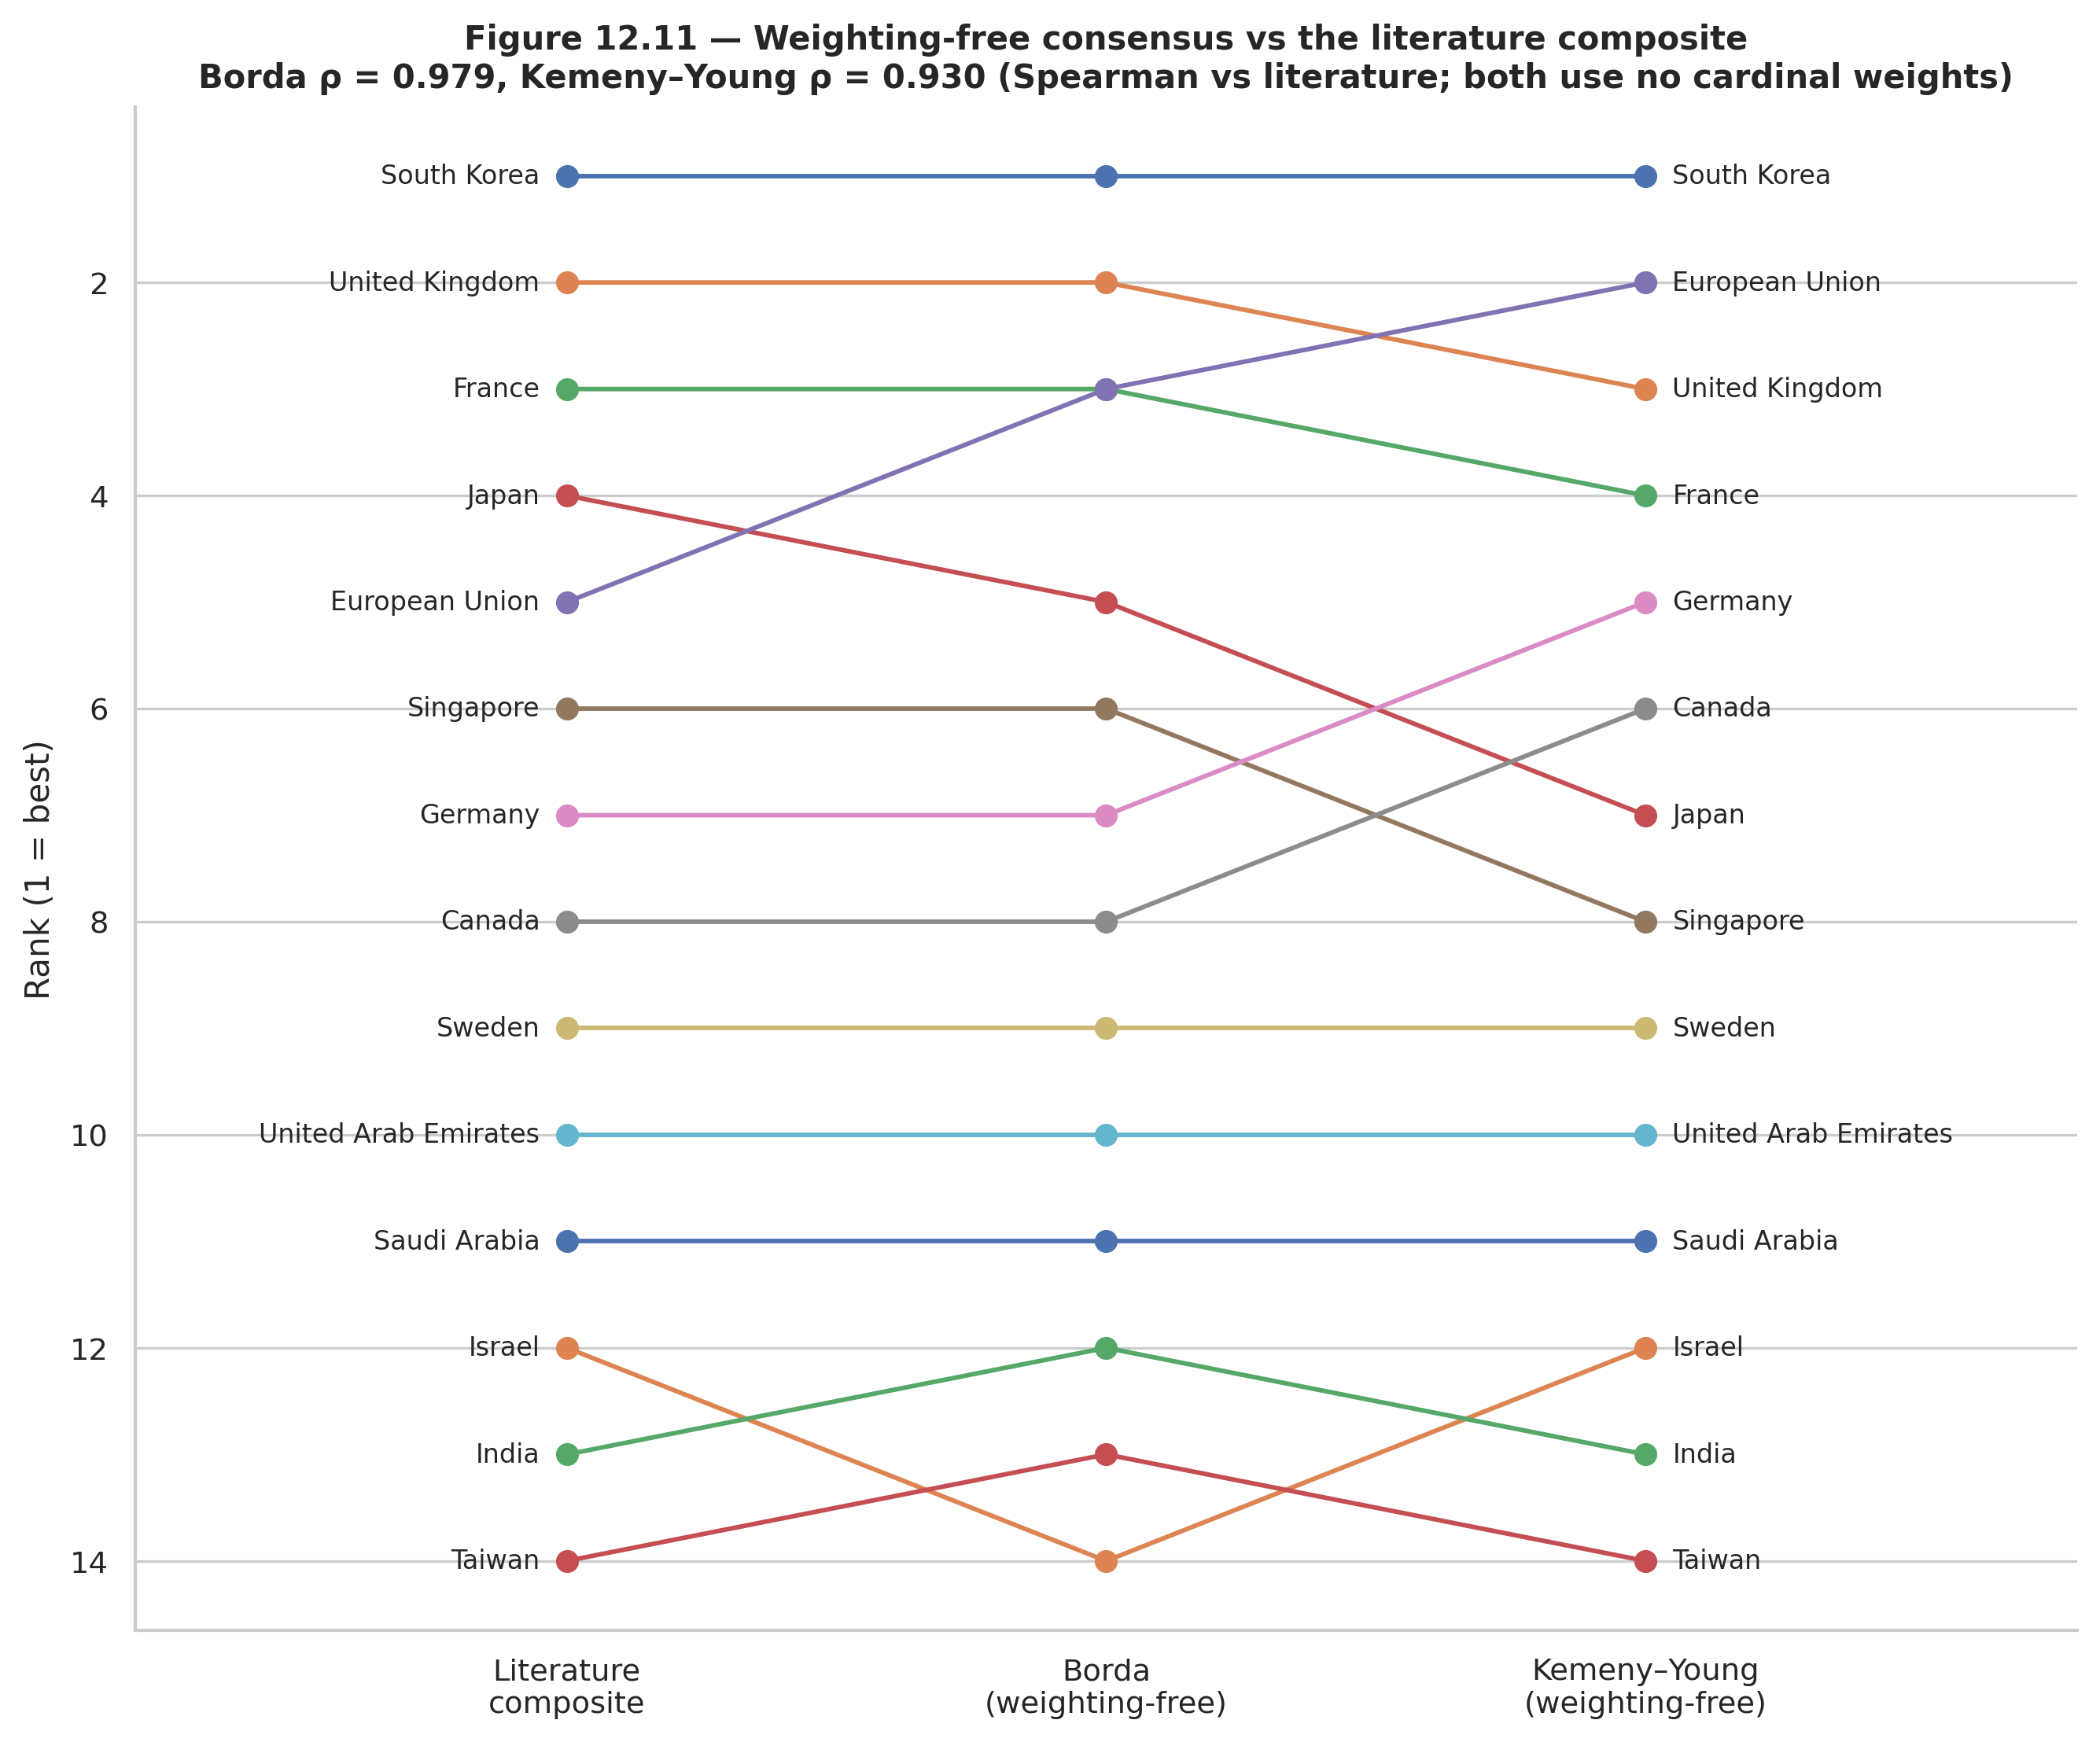
\includegraphics[width=0.78\textwidth]{figures/fig12_11_rank_aggregation.png}
\caption{Weighting-free consensus ranking. The literature composite rank versus the Borda count and the exact Kemeny--Young median ranking, each aggregating the fourteen indicator ballots with no cardinal weights. Source: \texttt{outputs/rank\_aggregation.csv}.}
\label{fig:rankagg}
\end{figure}

\begin{table}[t]
\centering
\caption{Per-vector preparedness scores and ranks. Higher score $=$ better prepared; signed $z$-scale, interpretable within a vector only. Source: \texttt{outputs/vulnerability\_overlay.csv}.}
\label{tab:vuln}
\small
\begin{tabular}{@{}lcccccc@{}}
\toprule
\textbf{Country} & \textbf{Cyber} & \textbf{Rk} & \textbf{CBRN} & \textbf{Rk} & \textbf{Infl.} & \textbf{Rk} \\
\midrule
South Korea           &  0.78 & 1  &  0.88 & 1  &  0.70 & 1 \\
United Kingdom        &  0.67 & 2  &  0.80 & 2  &  0.69 & 2 \\
Singapore             &  0.47 & 3  &  0.26 & 6  &  0.53 & 3 \\
European Union        &  0.46 & 4  &  0.55 & 4  &  0.22 & 6 \\
France                &  0.43 & 5  &  0.59 & 3  &  0.37 & 4 \\
Japan                 &  0.32 & 6  &  0.35 & 5  &  0.32 & 5 \\
Canada                &  0.06 & 7  &  0.14 & 7  & -0.11 & 9 \\
Germany               &  0.00 & 8  &  0.03 & 8  & -0.03 & 8 \\
Sweden                & -0.10 & 9  & -0.31 & 9  &  0.17 & 7 \\
United Arab Emirates  & -0.27 & 10 & -0.49 & 10 & -0.17 & 10 \\
Saudi Arabia          & -0.44 & 11 & -0.57 & 11 & -0.38 & 11 \\
Israel                & -0.65 & 12 & -0.74 & 13 & -0.65 & 13 \\
Taiwan                & -0.69 & 13 & -0.91 & 14 & -0.46 & 12 \\
India                 & -1.03 & 14 & -0.59 & 12 & -1.19 & 14 \\
\bottomrule
\end{tabular}
\end{table}

\begin{figure}[t]
\centering
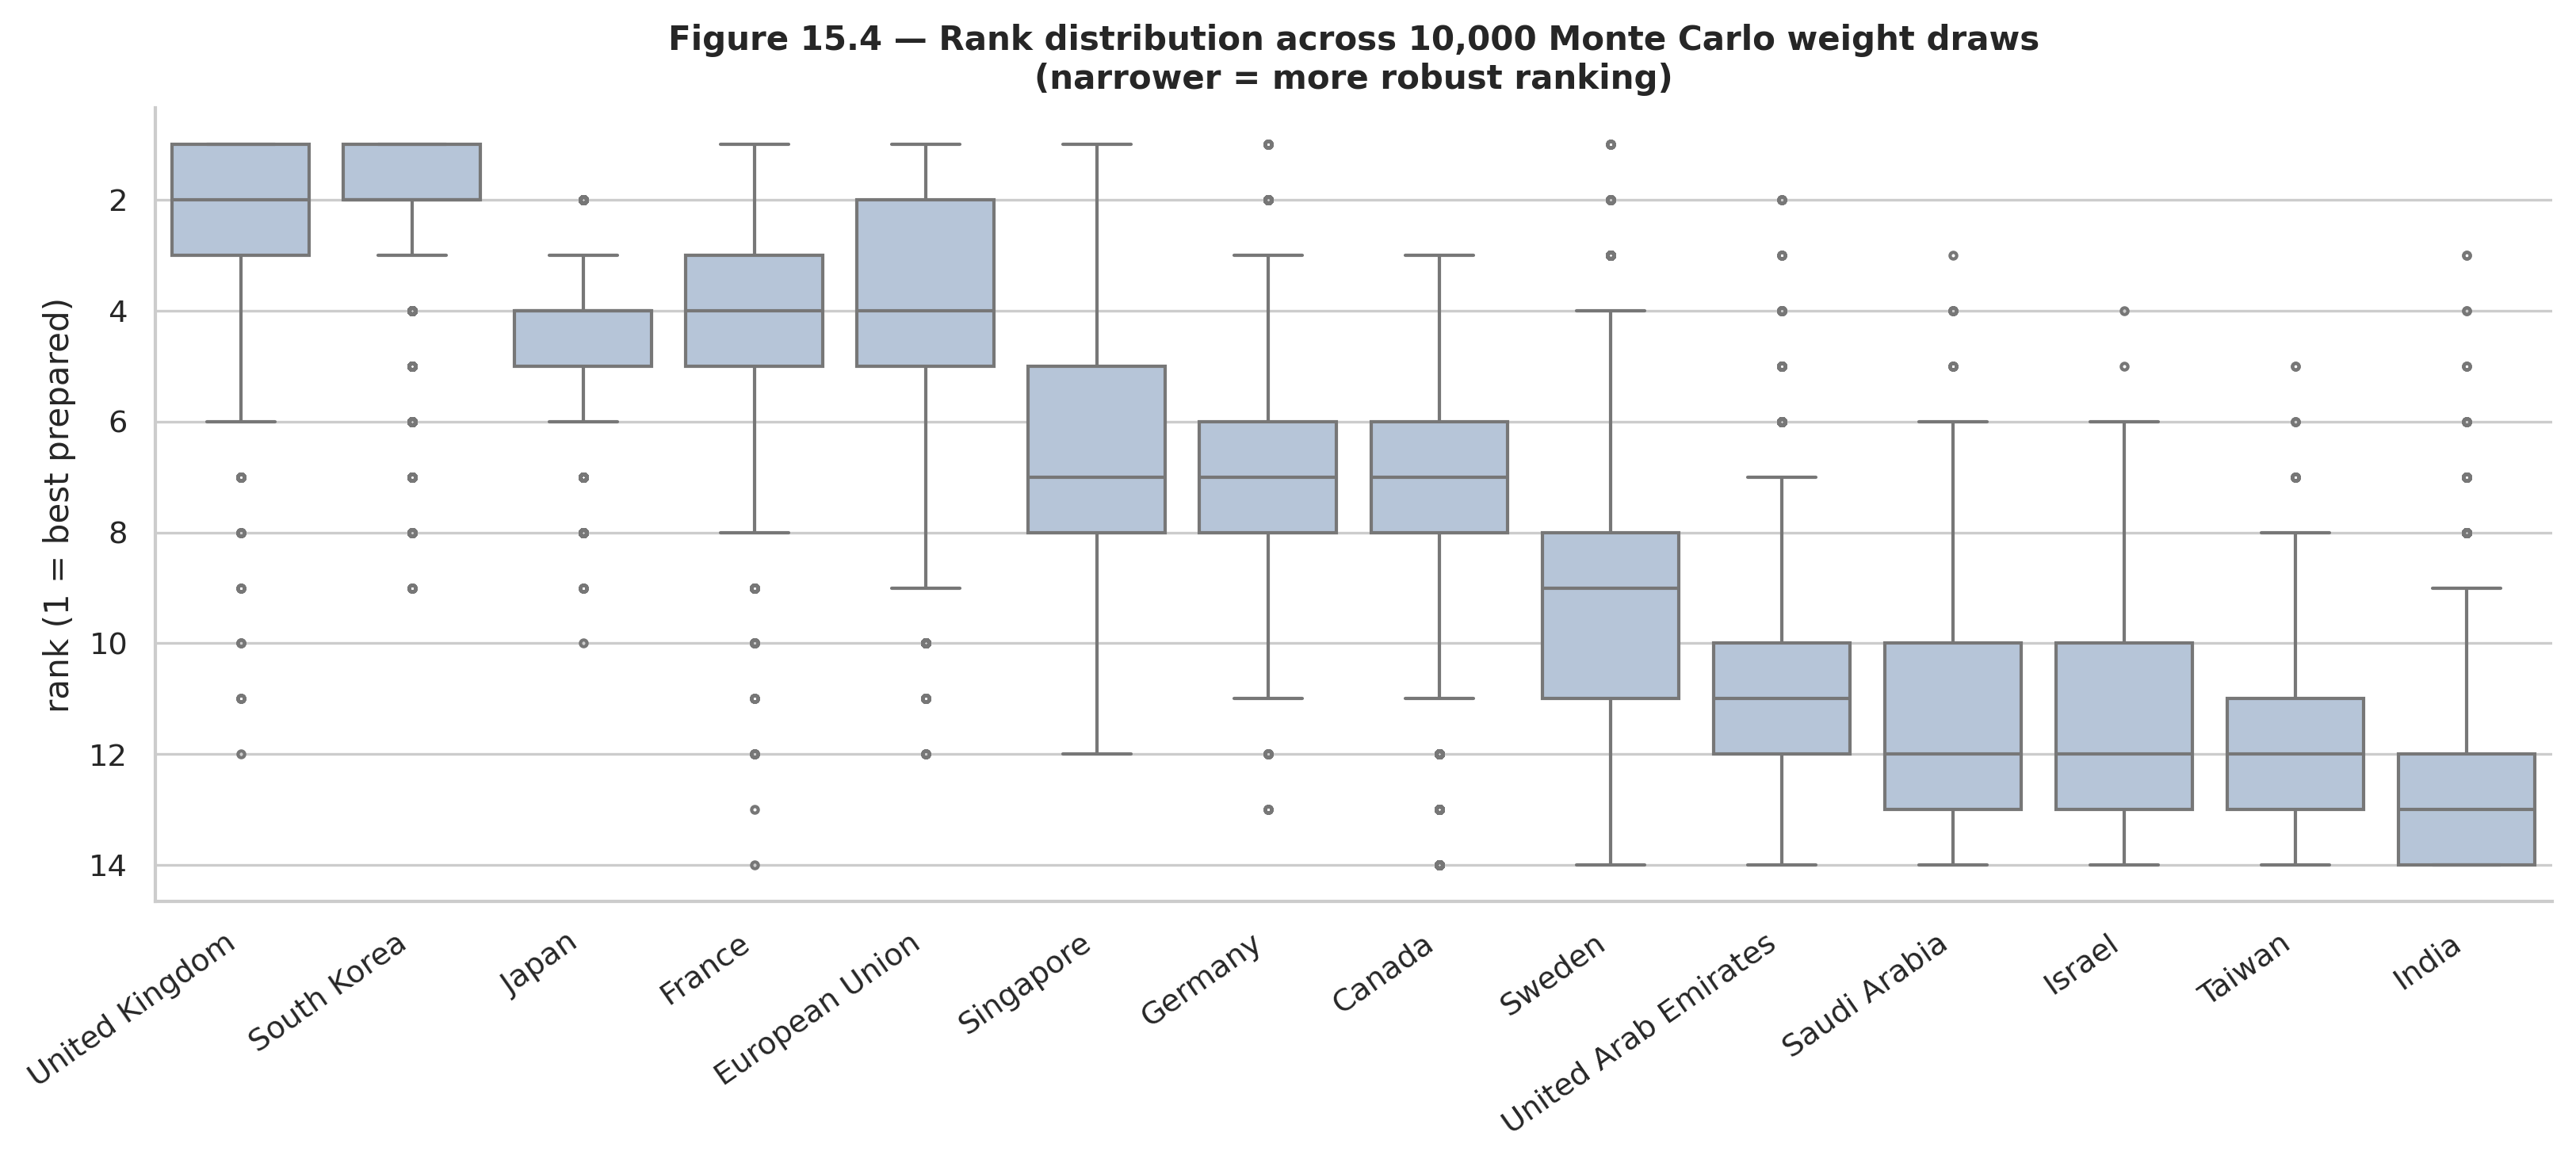
\includegraphics[width=0.9\textwidth]{figures/fig15_4_rank_distributions.png}
\caption{Per-country rank distribution across $10{,}000$ Monte Carlo weight draws (narrower $=$ more robust). Source: \texttt{outputs/sensitivity\_ranks.csv}.}
\label{fig:rankdist}
\end{figure}

\begin{figure}[t]
\centering
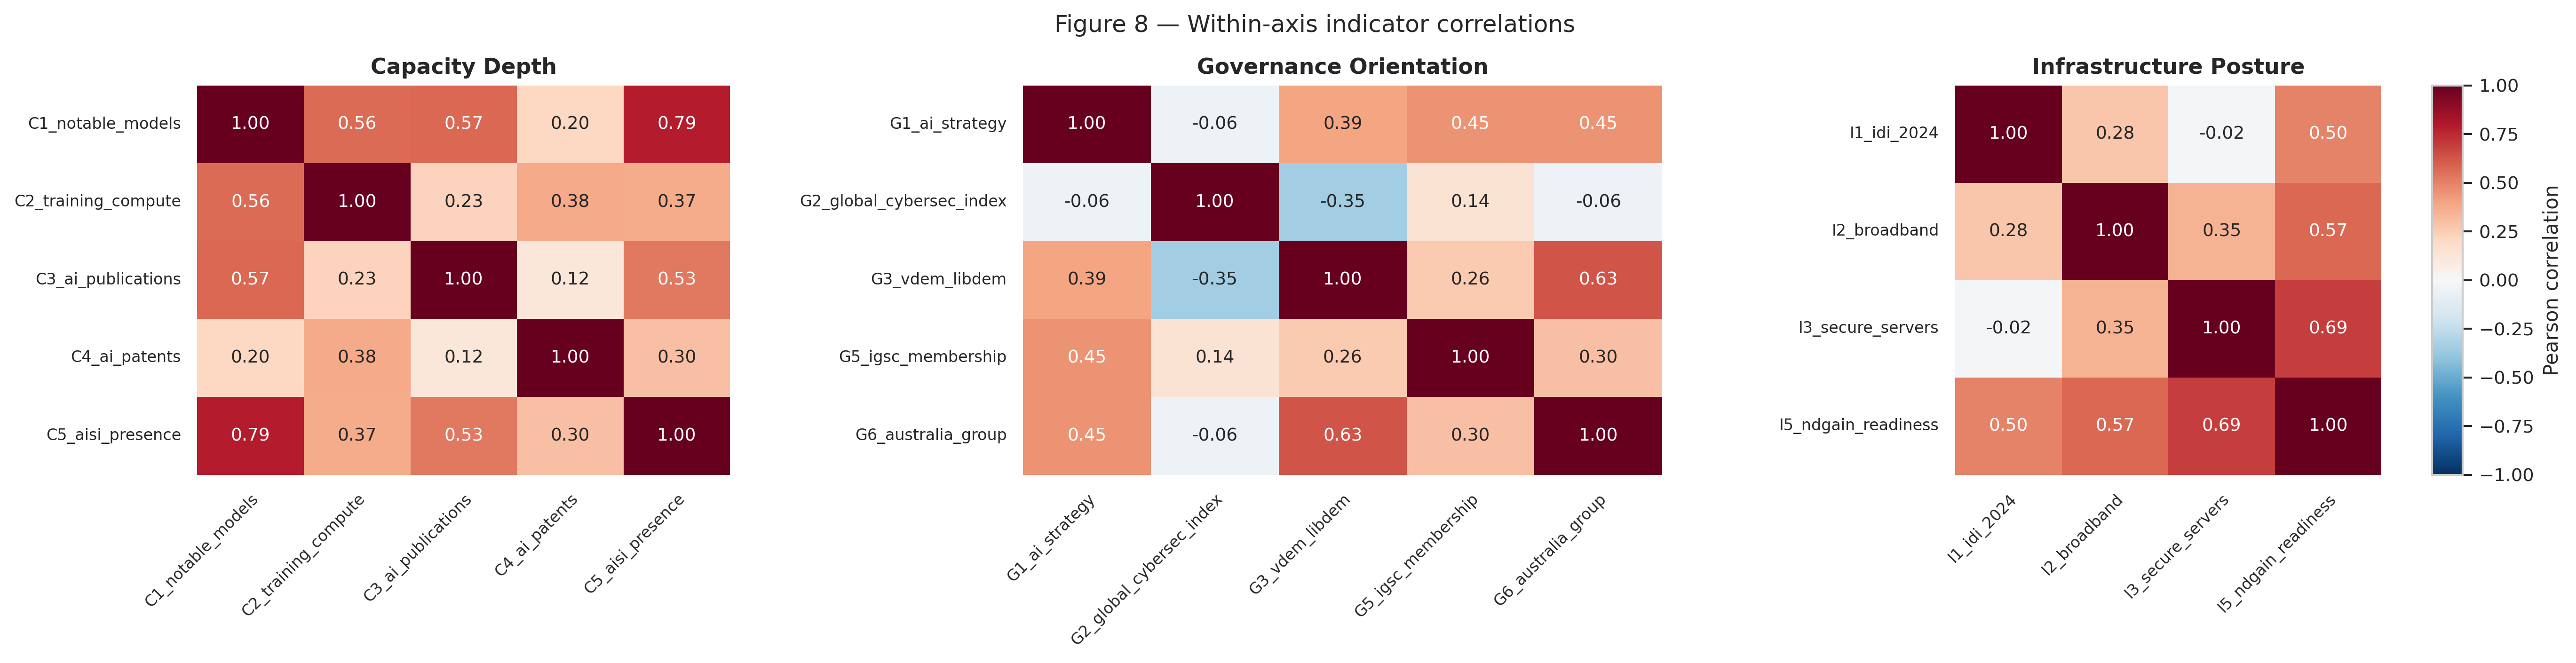
\includegraphics[width=0.97\textwidth]{figures/fig8_within_axis_correlations.png}
\caption{Within-axis indicator correlations (Pearson) for the three axes, with a shared colour scale. The governance panel shows the weak/negative association of the ITU GCI (G2) with its axis-mates that underlies the governance axis's lower internal consistency. Source: \texttt{outputs/cross\_axis\_correlations.csv}.}
\label{fig:withinaxis}
\end{figure}

\begin{figure}[t]
\centering
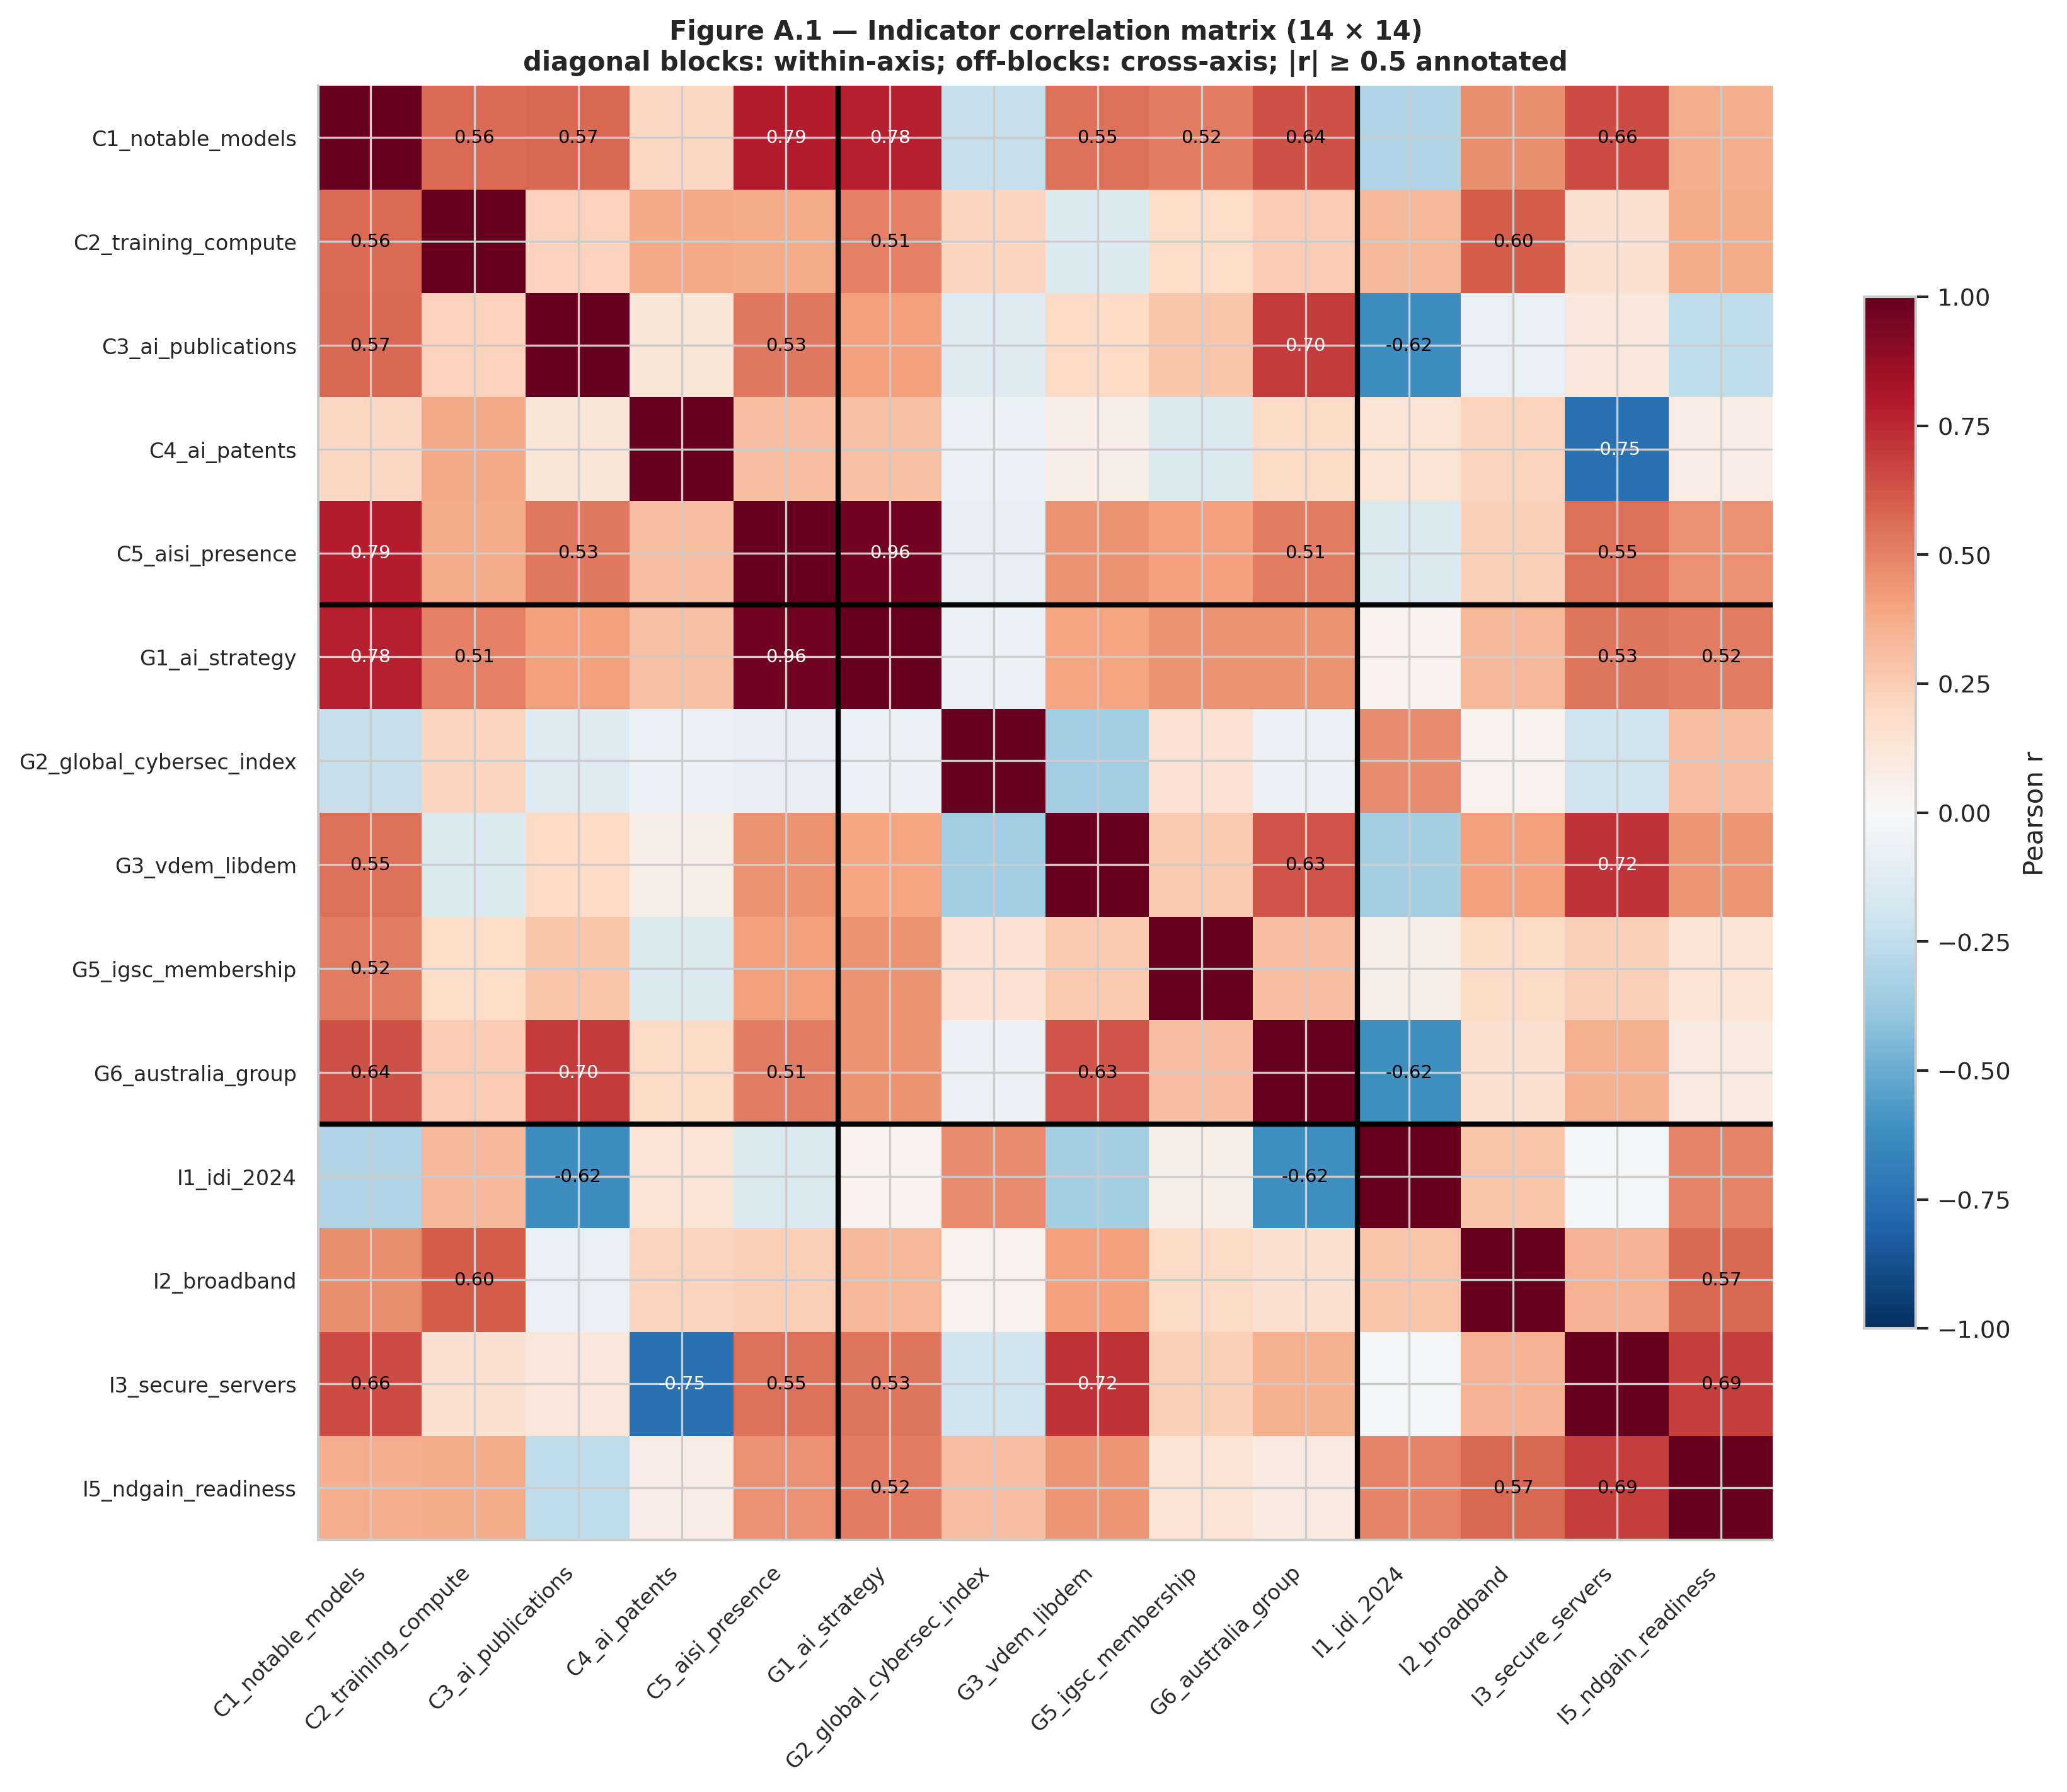
\includegraphics[width=0.82\textwidth]{figures/figA1_cross_axis_heatmap.png}
\caption{Full $14\times14$ indicator correlation matrix with axis-block separators; $|r|\geq0.5$ annotated. Diagonal blocks are within-axis; off-blocks are cross-axis. Source: \texttt{outputs/cross\_axis\_correlations.csv}.}
\label{fig:crossaxis}
\end{figure}

\begin{figure}[t]
\centering

\includegraphics[width=0.97\textwidth]{figures/fig14_2_hierarchical.png}
\caption{Hierarchical clustering at $k=3$ under Ward, complete, and average linkage. The complete- and average-linkage partitions are identical to the $k$-means partition (ARI $=1.0$); Ward is close (ARI $=0.727$). Source: \texttt{outputs/hierarchical\_ari.csv}.}
\label{fig:dendro}
\end{figure}

\begin{figure}[t]
\centering

\includegraphics[width=0.7\textwidth]{figures/fig15_1_axis_heatmap.png}
\caption{Per-country axis scores under the literature scheme ($z$-scale, clipped to $\pm1.5$), ordered by composite rank. Taiwan's infrastructure cell is column-mean-imputed. Source: \texttt{outputs/index\_baseline.csv}.}
\label{fig:axisheat}
\end{figure}

\begin{figure}[t]
\centering
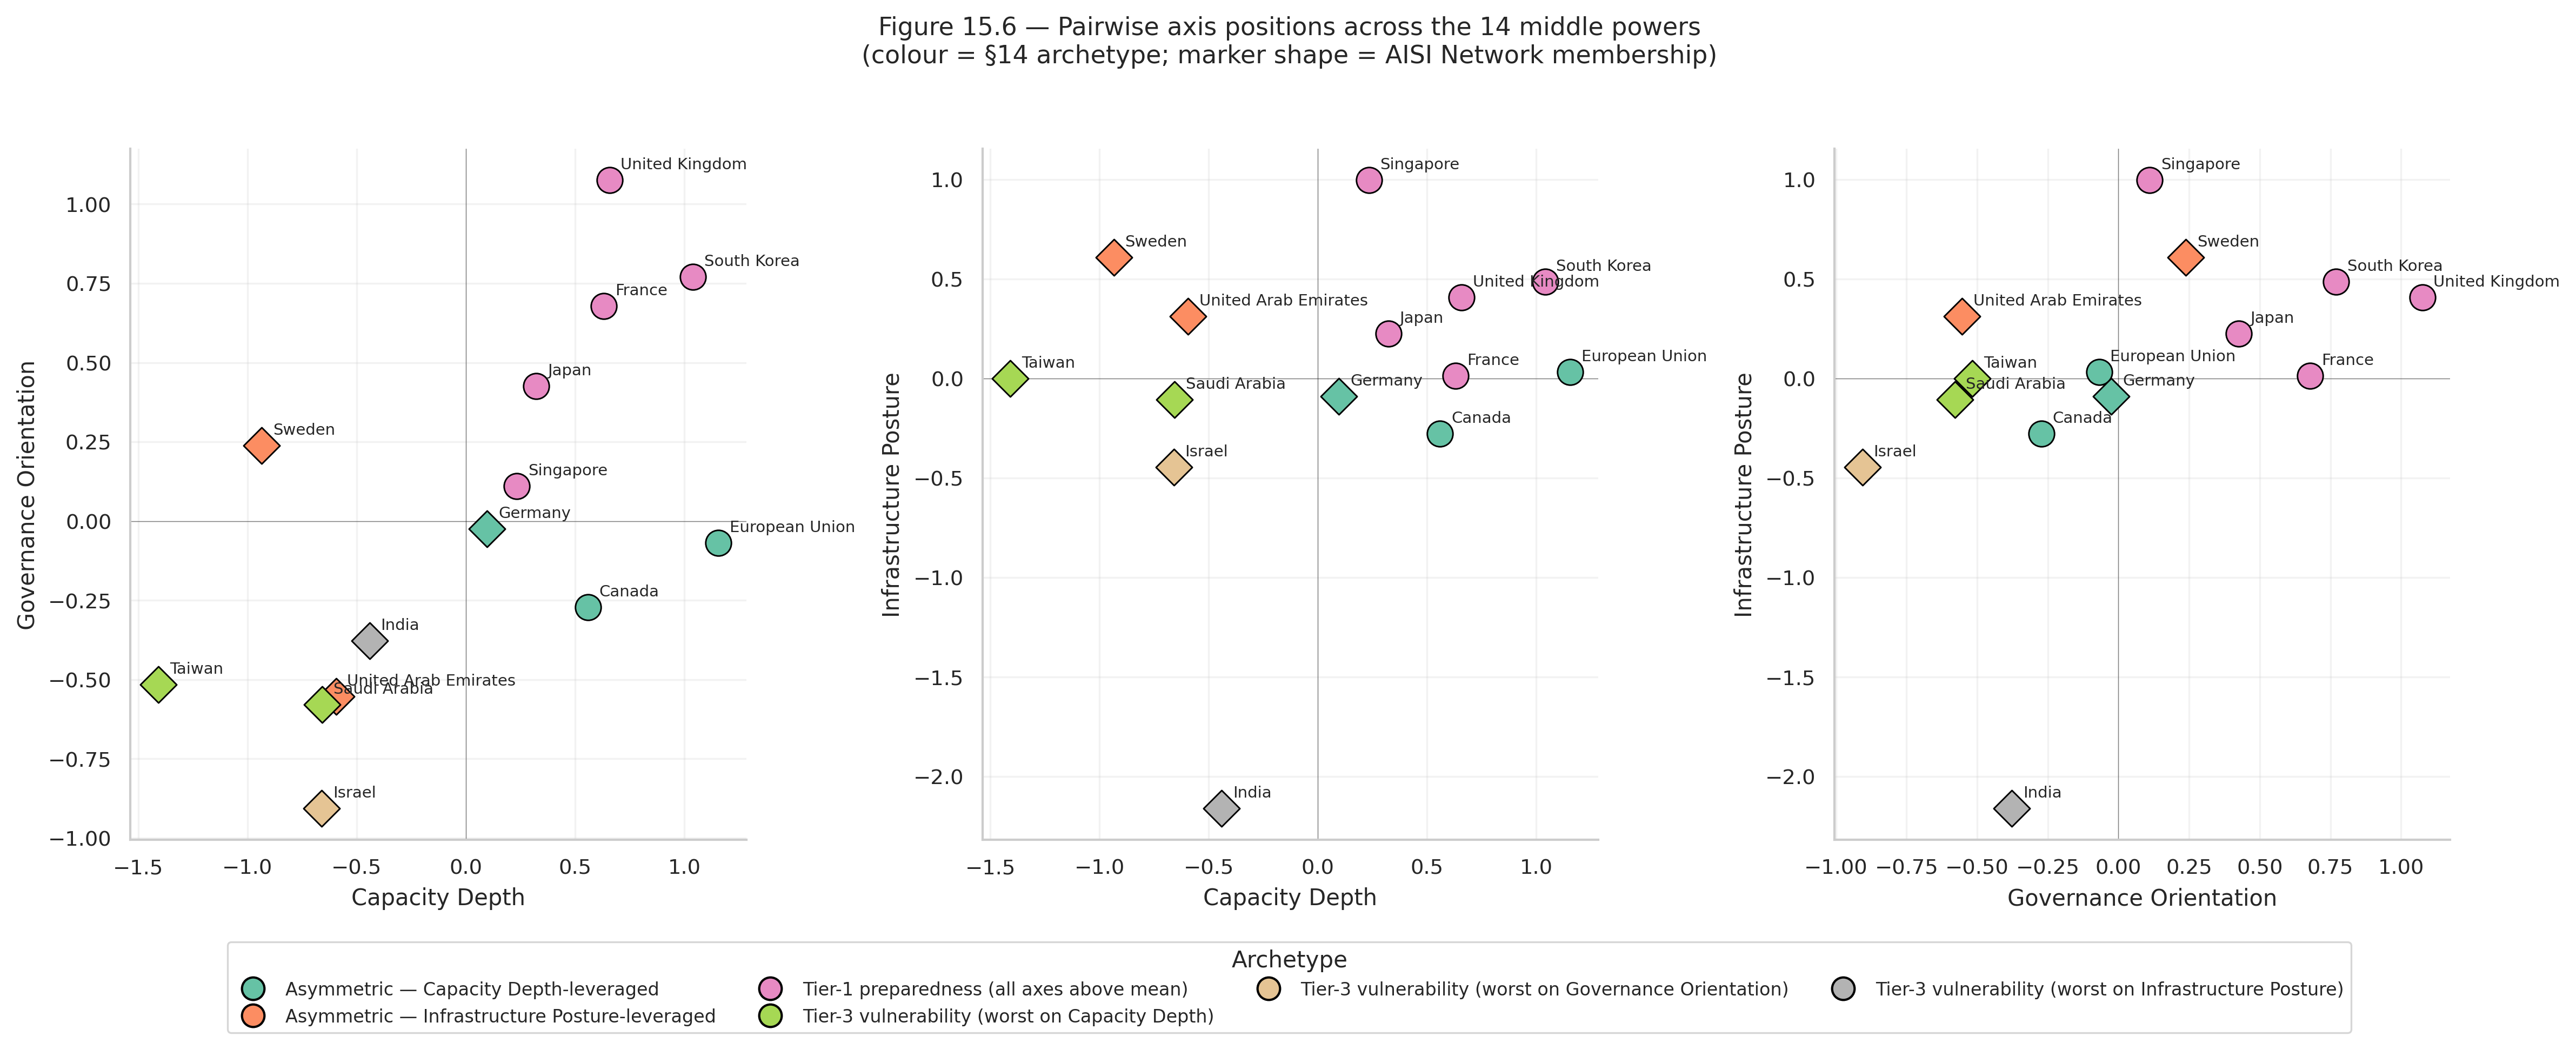
\includegraphics[width=0.97\textwidth]{figures/fig15_6_axis_scatter_matrix.png}
\caption{Pairwise axis positions across the 14 middle powers; colour: archetype; marker shape: AISI Network membership. Source: \texttt{outputs/index\_baseline.csv}.}
\label{fig:scatter}
\end{figure}

\begin{figure}[t]
\centering
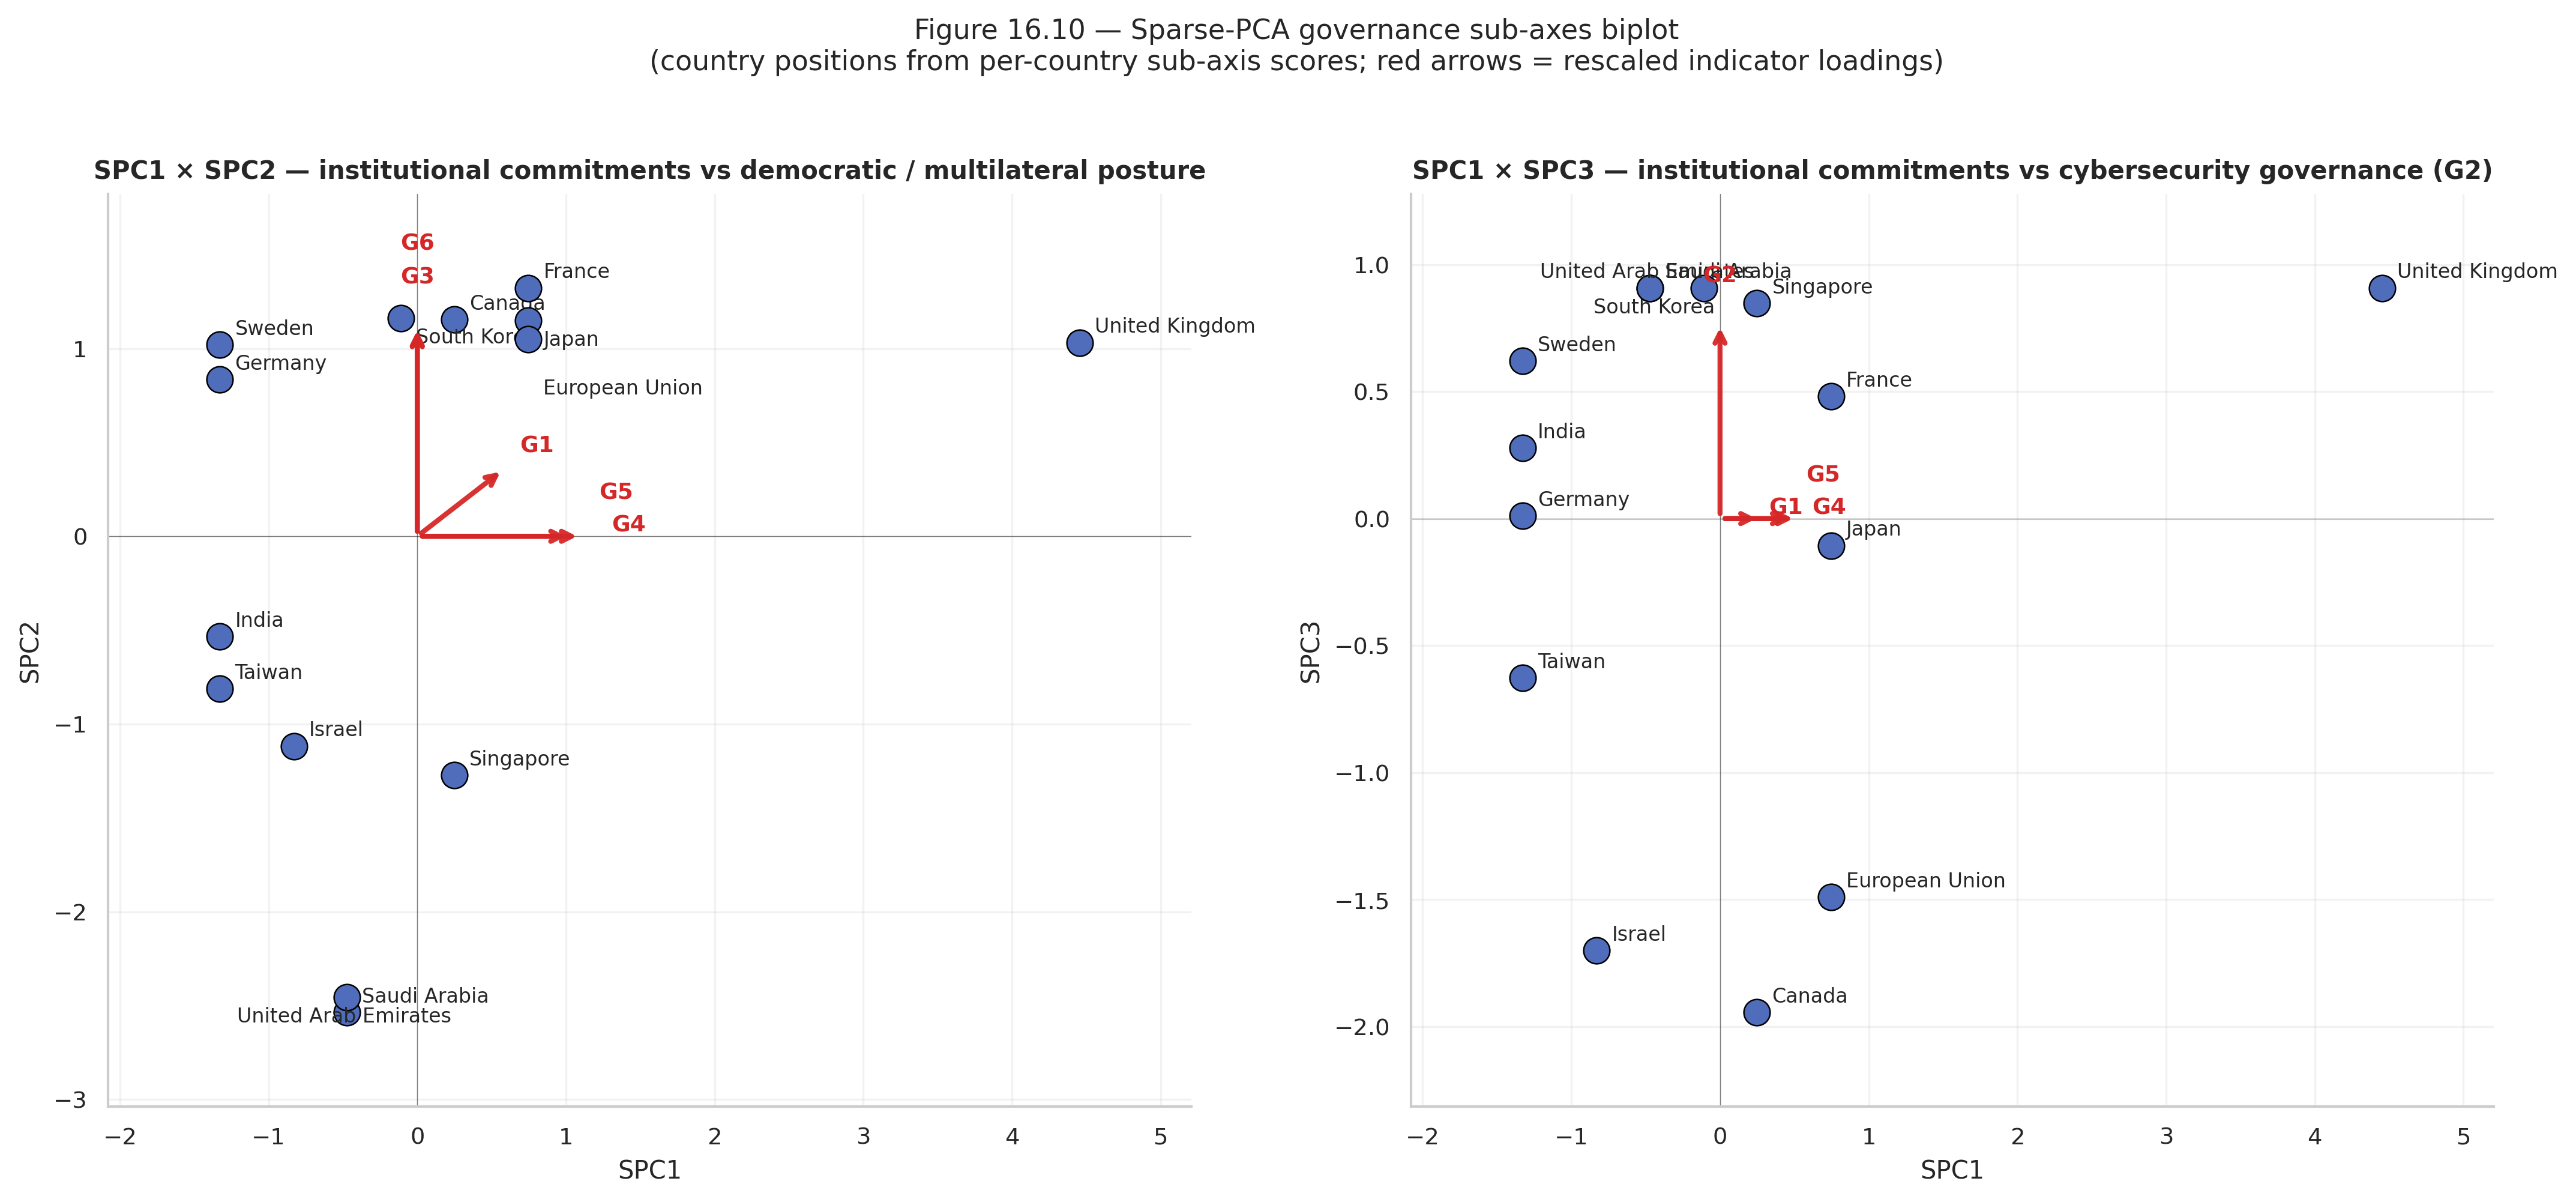
\includegraphics[width=0.95\textwidth]{figures/fig16_10_governance_biplot.png}
\caption{Sparse-PCA governance sub-axes biplot: country positions with rescaled indicator loadings (red arrows), decomposing the governance axis into institutional-commitment, democratic/multilateral, and cybersecurity sub-axes. Source: \texttt{outputs/governance\_subaxes.csv}.}
\label{fig:govbiplot}
\end{figure}

% ============================================================
\section{Interpretability}\label{app:interp}
% ============================================================
Figure~\ref{fig:shap} decomposes each country's composite into exact Shapley contributions per indicator (all $2^{14}$ coalitions; additivity verified to $10^{-6}$). Figure~\ref{fig:perm} reports permutation feature importance for the literature ranking. Training compute (C2) and ITU GCI (G2) are the most rank-disruptive indicators; secure servers (I3) and ND-GAIN readiness (I5) the least. Figure~\ref{fig:shapint} reports the exact second-order Shapley interaction indices \citep{grabisch1999interaction} for every indicator pair, averaged over the fourteen countries: the within-axis pairs are the substitutive (negative) ones, while cross-axis pairs---including the much-discussed C5$\times$G1 ($+0.009$)---are weakly complementary, locating indicator redundancy firmly within rather than across axes.

\begin{figure}[t]
\centering

\includegraphics[width=0.92\textwidth]{figures/figB1_shap_heatmap.png}
\caption{Exact Shapley decomposition of the literature composite. Rows: countries by composite rank; columns: indicators; each row sums to the composite minus the universal baseline. Source: \texttt{outputs/shap\_attributions.csv}.}
\label{fig:shap}
\end{figure}

\begin{figure}[t]
\centering
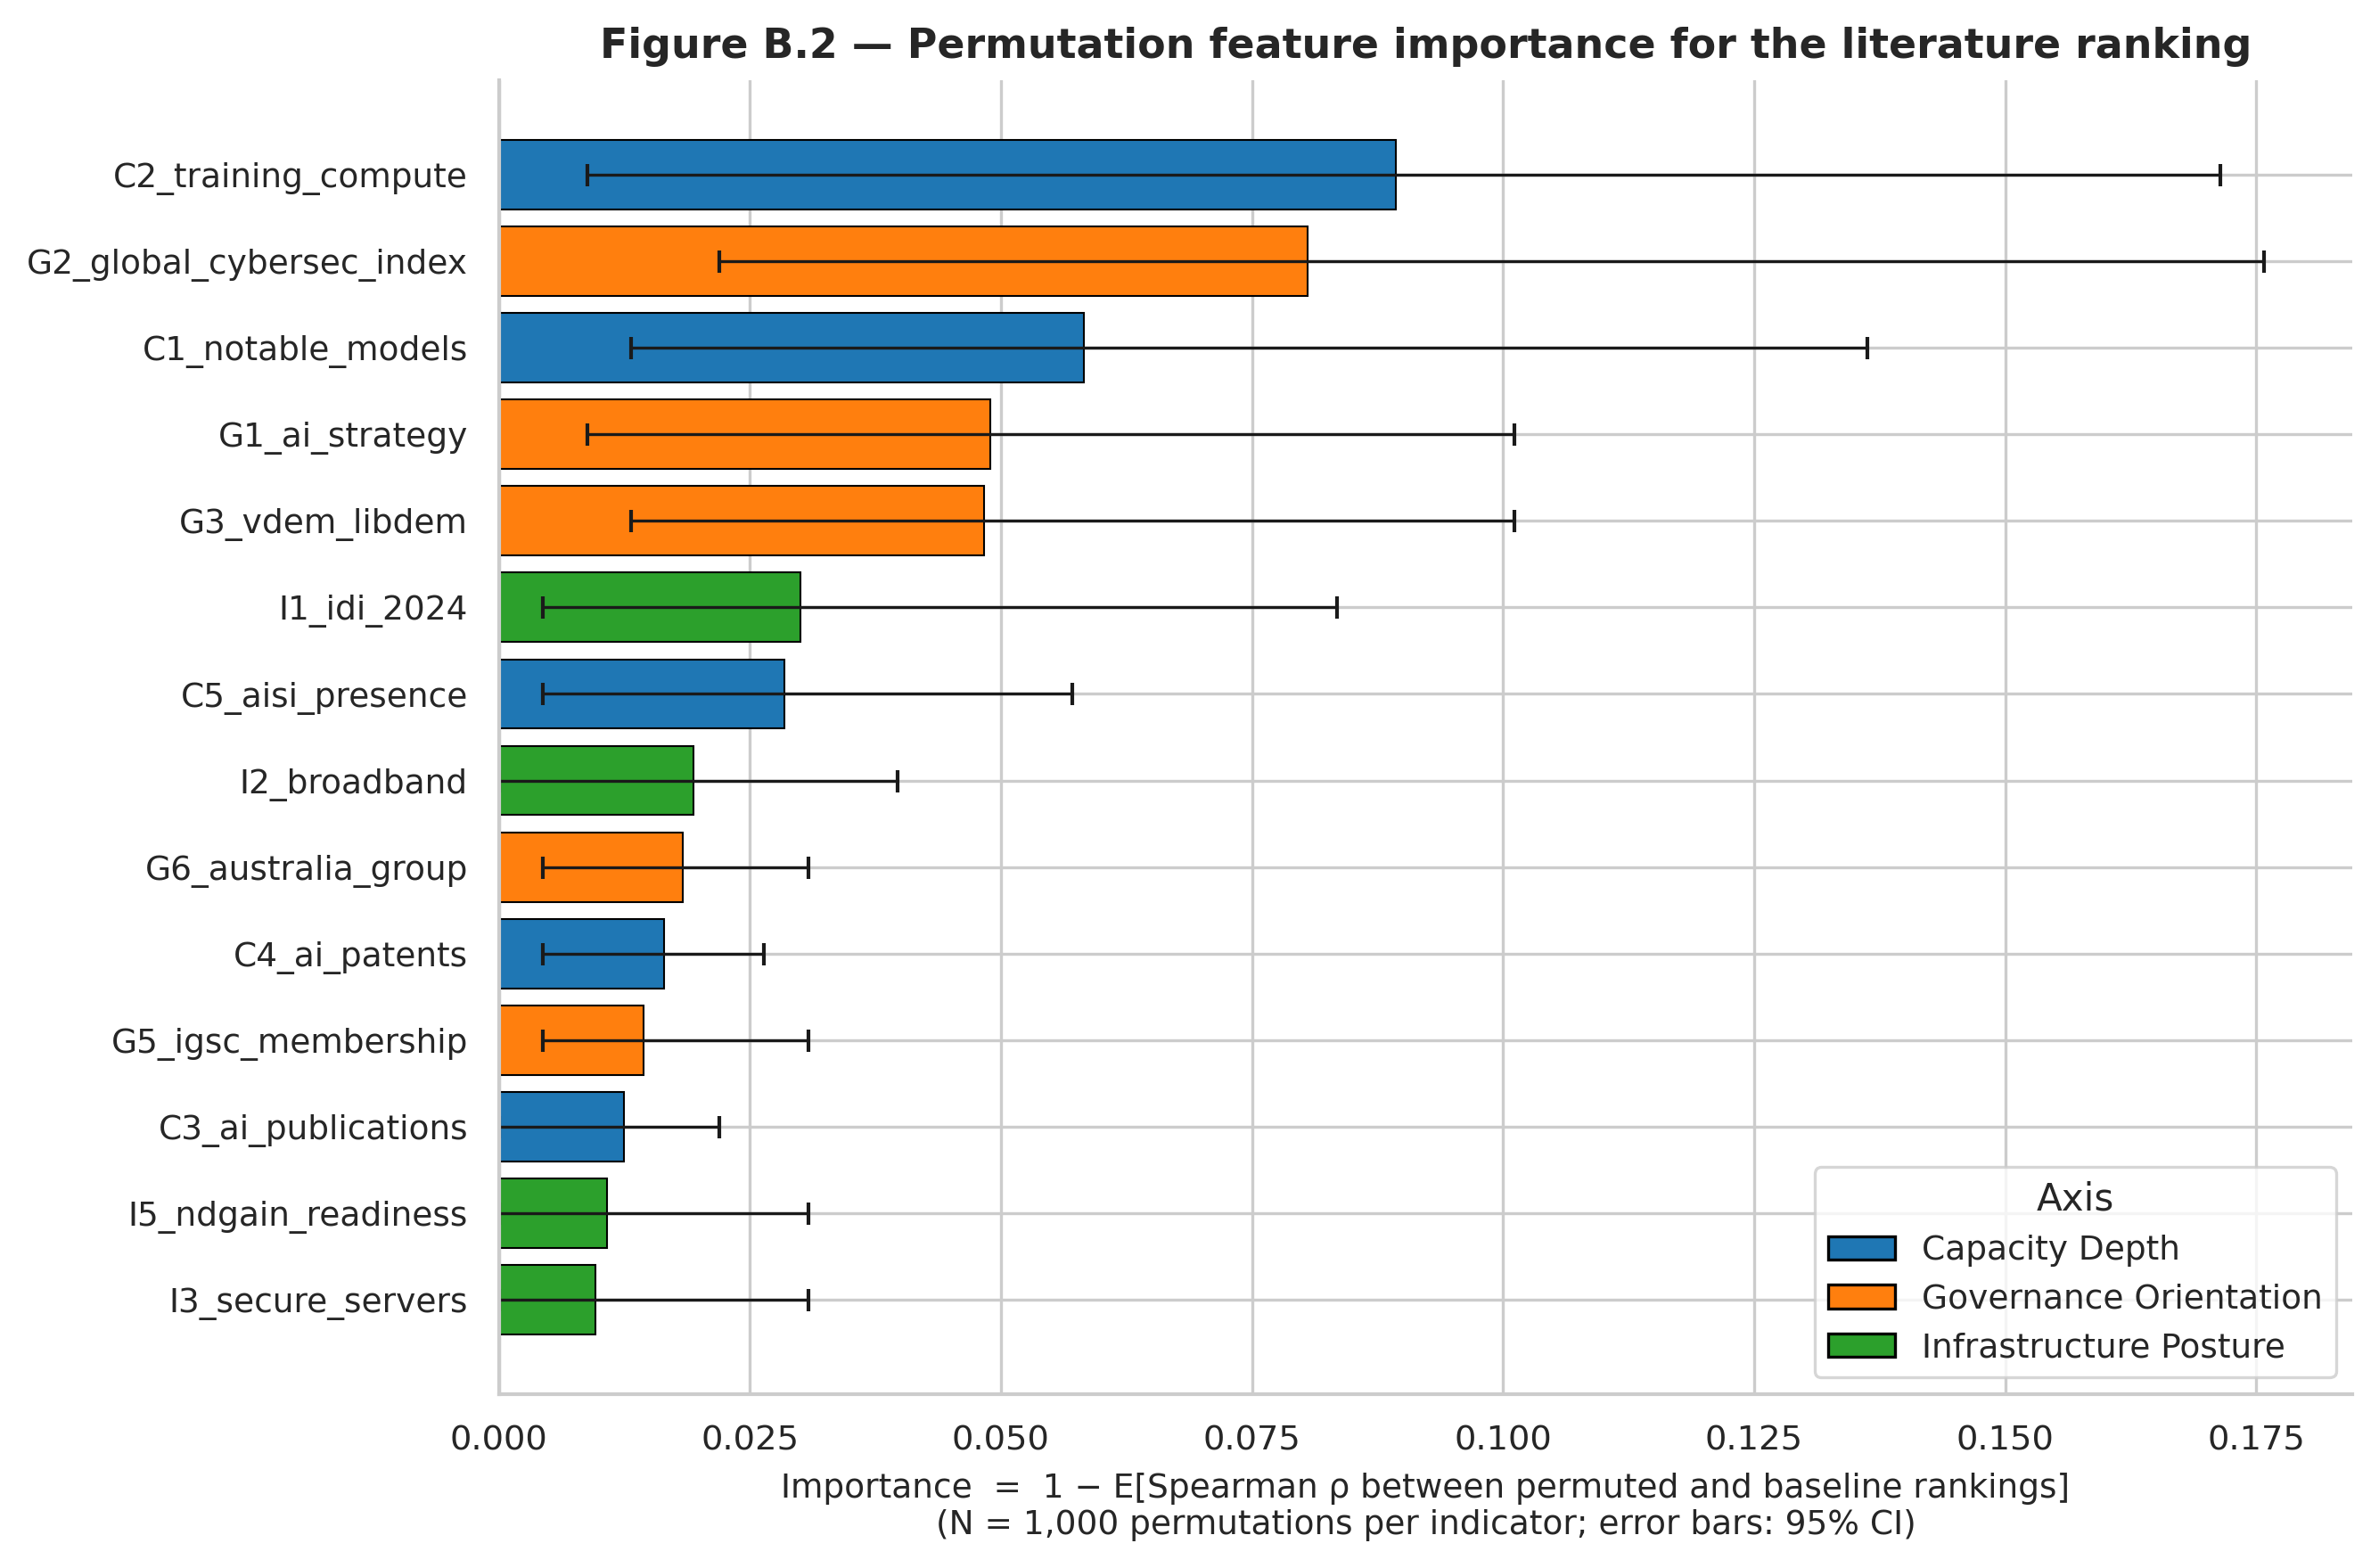
\includegraphics[width=0.8\textwidth]{figures/figB2_permutation_importance.png}
\caption{Permutation feature importance for the literature ranking (importance $= 1 - \mathbb{E}[\text{Spearman }\rho]$ between permuted and baseline rankings; $1{,}000$ permutations per indicator), coloured by axis. Source: \texttt{outputs/permutation\_importance.csv}.}
\label{fig:perm}
\end{figure}

\begin{figure}[t]
\centering
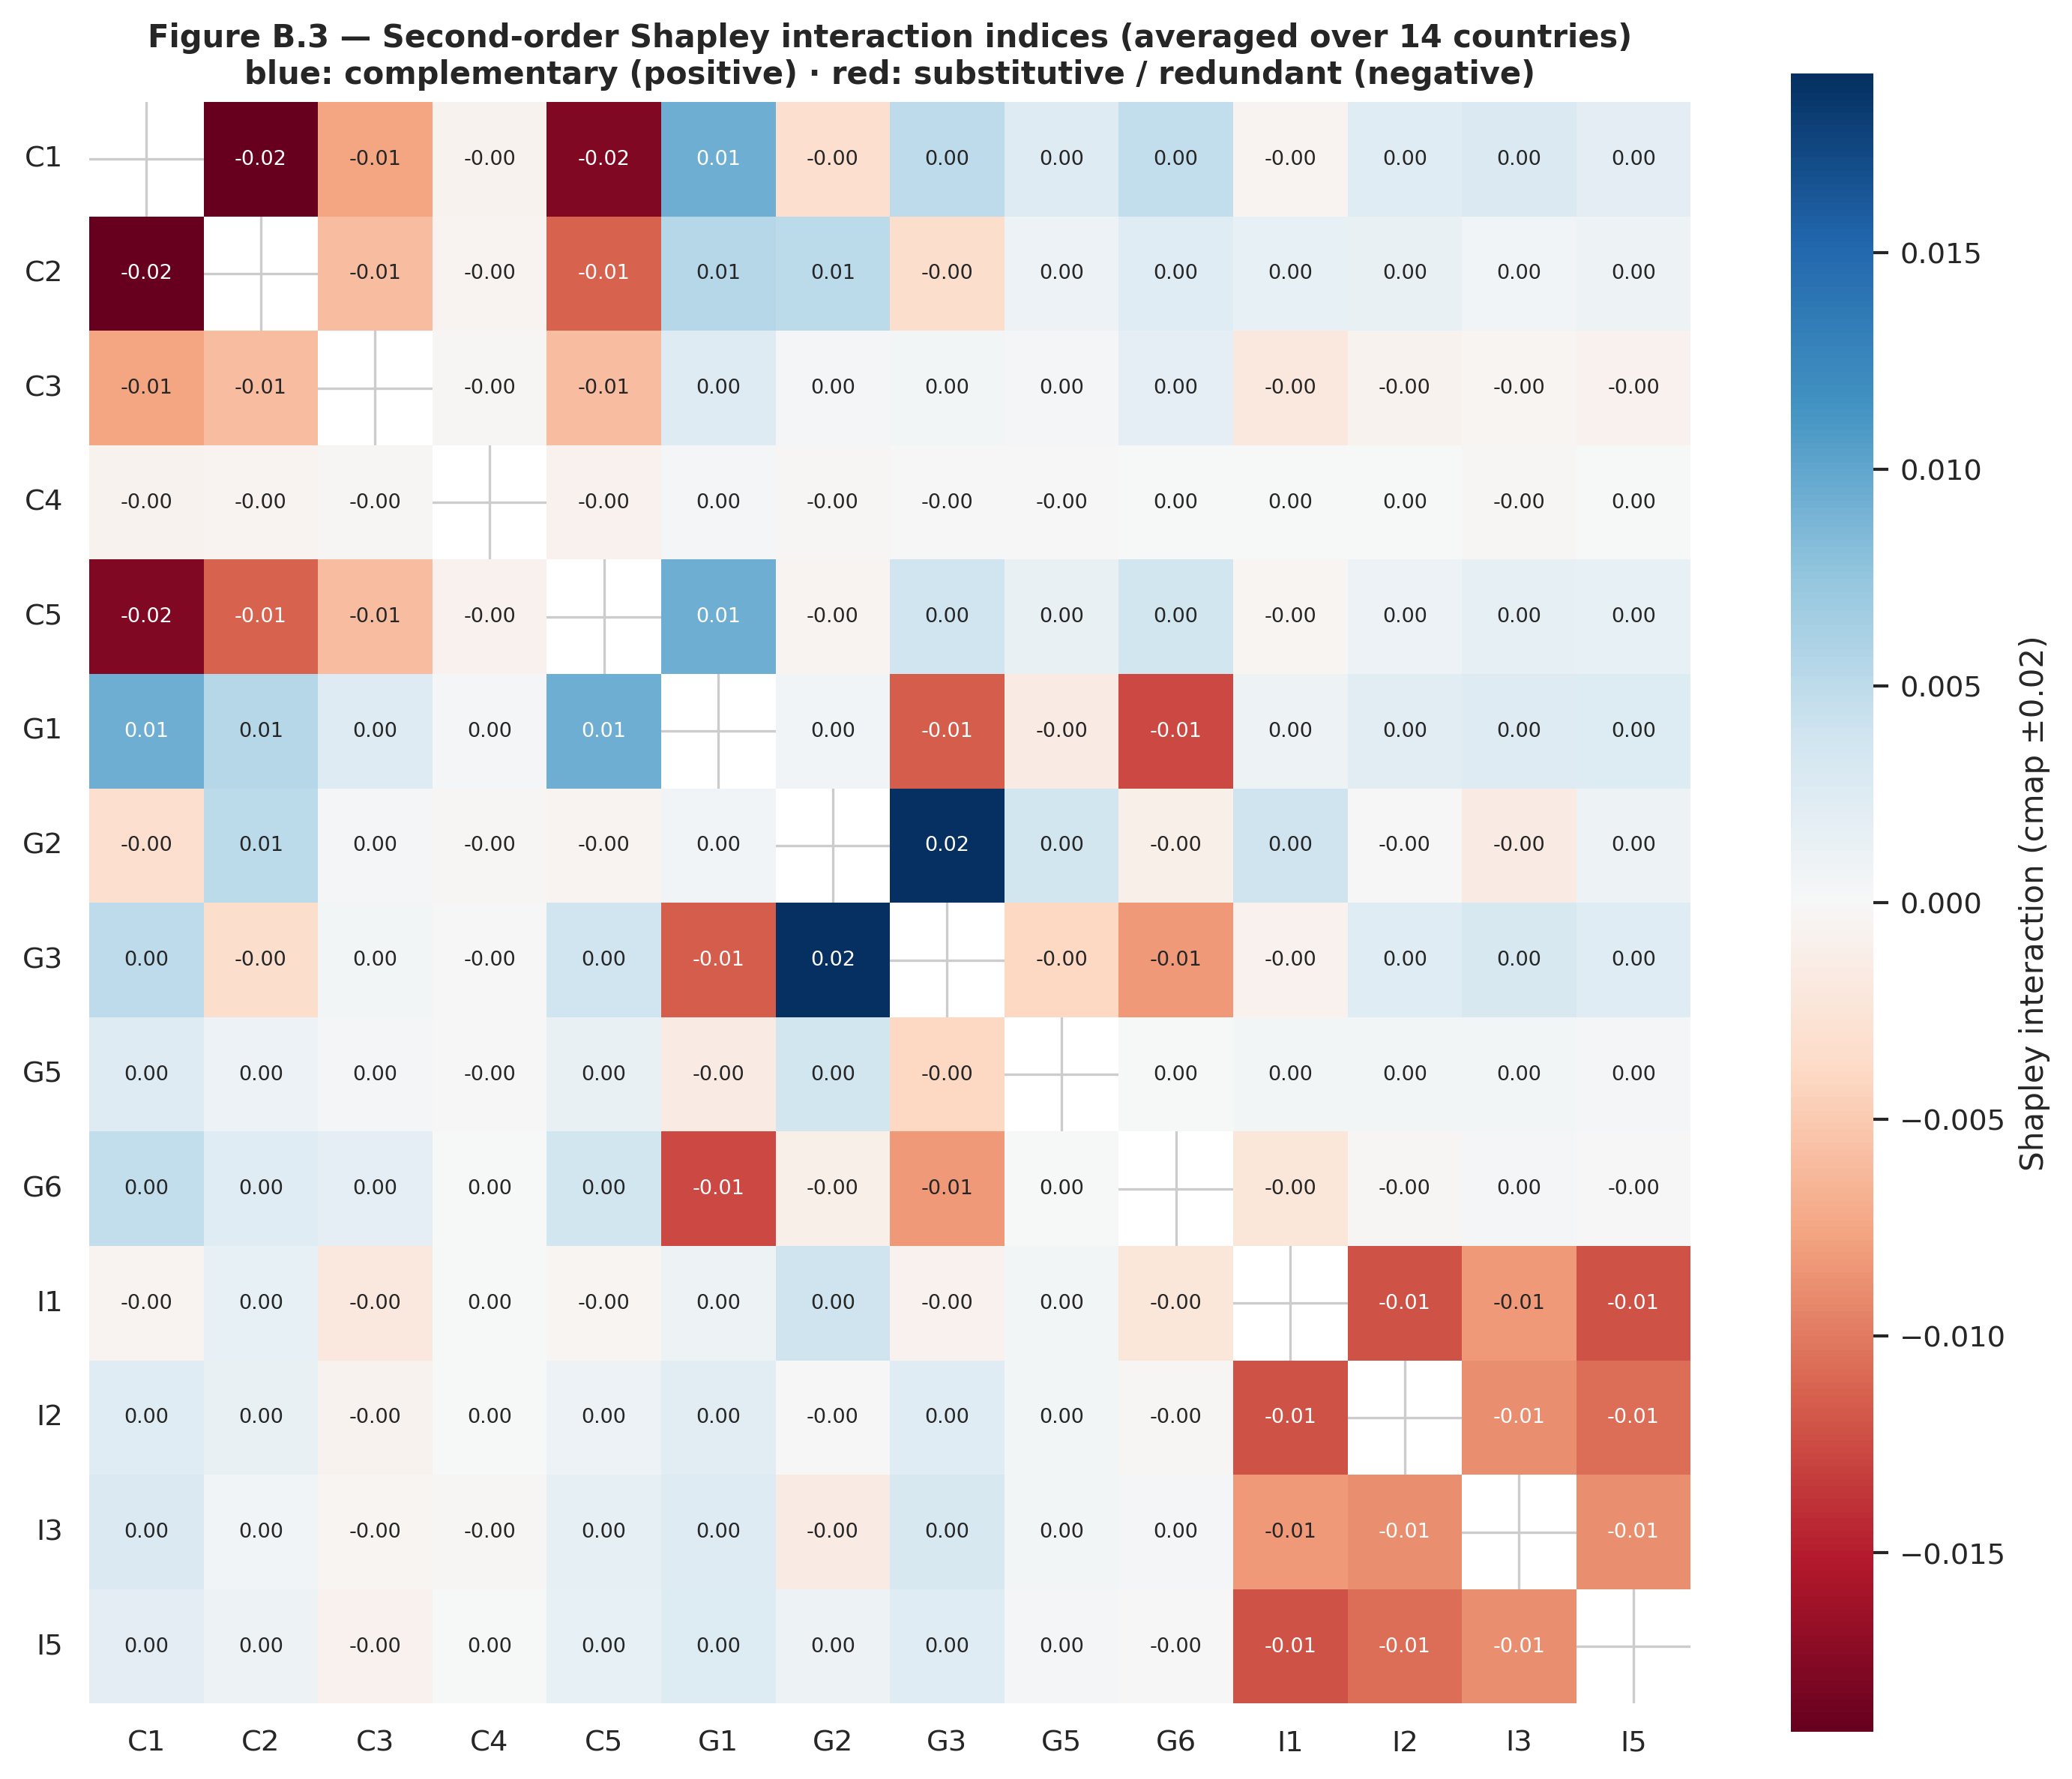
\includegraphics[width=0.82\textwidth]{figures/figB3_shap_interactions.png}
\caption{Second-order Shapley interaction indices for every indicator pair, averaged over the fourteen countries (all $2^{14}$ coalitions; \citealp{grabisch1999interaction}). Blue cells are complementary (positive), red cells substitutive/redundant (negative); the diagonal main effect is masked. Substitutive pairs are within-axis; cross-axis pairs, including C5$\times$G1, are weakly complementary. Source: \texttt{outputs/shap\_interactions.csv}.}
\label{fig:shapint}
\end{figure}

% ============================================================
\section{Reproducibility}\label{app:repro}
% ============================================================
All seven stochastic steps are seeded (\texttt{SEED $=$ 20260506}): the Monte Carlo weights, Horn's parallel-analysis null, the joint rank-uncertainty Monte Carlo, $k$-means, MDS, sparse PCA, and permutation importance. The leave-one-country-out re-clustering (\S\ref{subsec:mas} companion in \S\ref{sec:methods}) reuses the same seeded $k$-means; the Borda count and minimal-action-set enumeration are exact, and the Kemeny--Young median ranking is solved exactly by \texttt{scipy.optimize.milp} (HiGHS), deterministic within the pinned environment. With a pinned environment and the offline data snapshot (\texttt{MPAPI\_OFFLINE=1}), the thirty-five output files (thirty-two CSV, three JSON) and all twenty-three figures reproduce byte-for-byte across successive executions, verified by hashing two consecutive offline runs. The notebook additionally reconstructs one country's composite end-to-end (asserted within $10^{-3}$) and verifies Shapley additivity (within $10^{-6}$). The analysis is built on the open scientific Python stack \citep{harris2020numpy,mckinney2010pandas,virtanen2020scipy,pedregosa2011scikit,hunter2007matplotlib,waskom2021seaborn}.

\end{document}
